\documentclass[aspectratio=169,11pt]{beamer}

% ---- Minimalist theme (matches midway / implementation slides) ----
\usetheme{default}
\usecolortheme{default}
\setbeamertemplate{navigation symbols}{}
\setbeamertemplate{frametitle continuation}{}
\setbeamertemplate{itemize items}[circle]
\setbeamertemplate{enumerate items}[default]

% ---- Font: TeX Gyre Heros ----
\usepackage[T1]{fontenc}
\usepackage{tgheros}
\renewcommand{\familydefault}{\sfdefault}
\usepackage{microtype}

% ---- Packages ----
\usepackage{amsmath}
\usepackage{amssymb}
\usepackage{booktabs}
\usepackage{array}
\usepackage{tikz}
\usepackage{xcolor}
\usepackage{hyperref}
\usetikzlibrary{arrows.meta,positioning,calc,fit,shapes.geometric,backgrounds,patterns}

% ---- Maastricht University colors ----
\definecolor{umdark}{HTML}{001C3D}
\definecolor{umorange}{HTML}{E84E10}
\definecolor{umlight}{HTML}{4A90C4}
\definecolor{umgray}{HTML}{6B7280}
\newcommand{\icite}[1]{{\footnotesize\color{umgray!85}#1}}

% ---- Apply colors to Beamer ----
\setbeamercolor{normal text}{fg=umdark}
\setbeamercolor{frametitle}{fg=umdark}
\setbeamercolor{title}{fg=umdark}
\setbeamercolor{subtitle}{fg=umgray}
\setbeamercolor{author}{fg=umgray}
\setbeamercolor{date}{fg=umgray}
\setbeamercolor{institute}{fg=umorange}
\setbeamercolor{itemize item}{fg=umorange}
\setbeamercolor{itemize subitem}{fg=umlight}
\setbeamercolor{enumerate item}{fg=umorange}
\setbeamercolor{block title}{bg=umdark,fg=white}
\setbeamercolor{block body}{bg=umdark!5,fg=umdark}
\setbeamercolor{block title alerted}{bg=umorange,fg=white}
\setbeamercolor{block body alerted}{bg=umorange!8,fg=umdark}
\setbeamercolor{block title example}{bg=umlight,fg=white}
\setbeamercolor{block body example}{bg=umlight!8,fg=umdark}

% ---- Frametitle style ----
\setbeamertemplate{frametitle}{%
  \vspace{0.35cm}%
  \noindent\hspace*{0pt}%
  \parbox{\textwidth}{%
    {\usebeamerfont{frametitle}\usebeamercolor[fg]{frametitle}\insertframetitle}%
    \vspace{2pt}\\%
    {\color{umorange}\rule{\textwidth}{1.2pt}}%
  }%
  \vspace{-2pt}%
}
\setbeamerfont{frametitle}{size=\large,series=\bfseries}
\setbeamersize{text margin left=0.7cm,text margin right=0.7cm}

% ---- Footline ----
\setbeamertemplate{footline}{%
  \hbox{%
    \begin{beamercolorbox}[wd=\paperwidth,ht=2.2ex,dp=1ex]{footline}%
      \hspace{1em}{\scriptsize\color{umgray}Final Presentation -- Carrier Origin and Steganographic Detectability}%
      \hfill%
      {\scriptsize\color{umgray}\insertframenumber/\inserttotalframenumber}%
      \hspace{1em}%
    \end{beamercolorbox}%
  }%
}

% ---- Shared TikZ styles ----
\tikzset{
  pstage/.style    = {rectangle, draw=umdark, fill=umdark!8, rounded corners=2pt,
                       minimum width=2.05cm, minimum height=0.85cm, align=center,
                       font=\scriptsize\bfseries\color{umdark}},
  pout/.style      = {font=\tiny\color{umgray}, align=center},
  parrow/.style    = {-Stealth, thick, umorange},
  srcbox/.style    = {rectangle, draw=umorange, fill=umorange!12, rounded corners=2pt,
                       minimum width=1.6cm, minimum height=0.55cm, align=center,
                       font=\scriptsize\bfseries\color{umdark}},
  capbox/.style    = {rectangle, draw=umlight, fill=umlight!12, rounded corners=2pt,
                       minimum width=4.4cm, minimum height=0.55cm, align=center,
                       font=\scriptsize\itshape\color{umdark}},
  condcell/.style  = {rectangle, draw=umdark!25, fill=white,
                       minimum width=0.42cm, minimum height=0.32cm, font=\tiny},
  bitcell/.style   = {rectangle, draw=umdark!60, fill=white,
                       minimum width=0.40cm, minimum height=0.45cm, font=\scriptsize\ttfamily, inner sep=1pt},
  bitlsb/.style    = {rectangle, draw=umorange, line width=0.9pt, fill=umorange!15,
                       minimum width=0.40cm, minimum height=0.45cm, font=\scriptsize\ttfamily\bfseries, inner sep=1pt},
  dctcell/.style   = {rectangle, draw=umdark!25, fill=white,
                       minimum width=0.36cm, minimum height=0.36cm, font=\tiny\color{umdark}},
  dctused/.style   = {rectangle, draw=umorange, fill=umorange!18, line width=0.4pt,
                       minimum width=0.36cm, minimum height=0.36cm, font=\tiny\color{umdark}},
  dctskip/.style   = {rectangle, draw=umgray, fill=umgray!22, line width=0.4pt,
                       minimum width=0.36cm, minimum height=0.36cm, font=\tiny\color{umgray}},
}

% ---- Metadata ----
\title{Does the Source of Carrier Image Affect\\Steganographic Detectability?}
\subtitle{Final Presentation}
\newcommand{\teamauthors}{Abdul Moiz Akbar \;|\; Daria Gjonbalaj \;|\; Nico Muller-Spath\\Jimena Narvaez del Cid \;|\; David Wicker \;|\; Nikolas Zouros}
\author[Project 2.2 Team]{Project 2.2 Team}
\institute{Department of Advanced Computing Sciences\\Maastricht University}
\date{Project 2.2 \;|\; May 2026}

\begin{document}

% ============================================================
% 1. Opening
% ============================================================
\begin{frame}[plain]
\vfill
\begin{center}
{\color{umorange}\rule{0.42\textwidth}{2pt}}\\[12pt]
{\LARGE\bfseries\color{umdark}\inserttitle}\\[10pt]
{\normalsize\color{umgray}\insertsubtitle}\\[16pt]
{\small\color{umdark}\teamauthors}\\[8pt]
{\small\color{umorange}\insertinstitute}\\[8pt]
{\footnotesize\color{umgray}\insertdate}\\[12pt]
{\color{umorange}\rule{0.42\textwidth}{2pt}}
\end{center}
\vfill
\end{frame}

% ============================================================
% 2. Agenda
% ============================================================
\begin{frame}{Agenda}
\small
\begin{enumerate}
\item Motivation recap
\item Research questions
\item Experimental design and methods
\item Statistical analysis
\item Results across RQ1--RQ5
\item Limitations and contribution
\end{enumerate}
\end{frame}

% ============================================================
% 3. Motivation recap
% ============================================================
\section{Motivation}
\begin{frame}{Motivation Recap}
\small
\begin{itemize}
\item Steganalysis detectability depends on carrier-image statistics, not only on embedding logic \icite{(Petitcolas et al., 1999; Fridrich \& Kodovsky, 2012).}
\item Photographic carriers dominate benchmarks, yet diffusion outputs are now everywhere and carry distinct statistical traces \icite{(Corvi et al., 2023).}
\item Closest prior work studies AI carriers under adaptive embedding and reports $P_E$, not AUC \icite{(M\'ereur et al., 2024).}
\end{itemize}
\vspace{0.1cm}
\begin{alertblock}{Core question}
Do detectors validated on photographs remain equally effective when the carrier is ML-generated, under identical embedding settings?
\end{alertblock}
\end{frame}

% ============================================================
% 4. Research Questions
% ============================================================
\section{Research Questions}
\begin{frame}{Research Questions}
\scriptsize
\begin{columns}[T]
\begin{column}{0.49\textwidth}
\begin{block}{RQ1 (Primary, confirmatory)}
Does carrier source (real vs.\ pooled ML) affect detectability under matched embedding settings?
\end{block}
\begin{block}{RQ2 (Primary, confirmatory)}
Within ML carriers, does the choice of generator (SDXL vs.\ FLUX) change detectability?
\end{block}
\begin{block}{RQ3 (Exploratory)}
Does payload size change the detectability gap between real and ML carriers?
\end{block}
\end{column}
\begin{column}{0.49\textwidth}
\begin{block}{RQ4 (Exploratory)}
Do the spatial (LSB+PNG) and frequency (DCT-LSB+JPEG) branches show different carrier-source effects?
\end{block}
\begin{block}{RQ5 (Verification)}
Does AES-256-CBC payload encryption affect detectability? Expected null result.
\end{block}
\end{column}
\end{columns}
\end{frame}

% ============================================================
% 5. Experimental Design  (NEW: caption-matched diagram)
% ============================================================
\section{Experimental Design}
\begin{frame}{Caption-Matched Carriers, $3 \times 2 \times 3 \times 2$ Factorial}
\small
\begin{columns}[T]
\begin{column}{0.46\textwidth}
\vspace{-0.05cm}
\begin{center}
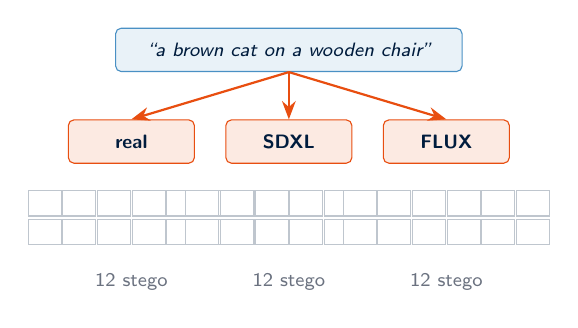
\begin{tikzpicture}[node distance=0.45cm and 0.25cm]
% Caption at top
\node[capbox] (cap) {``a brown cat on a wooden chair''};

% Three source nodes
\node[srcbox, below=0.6cm of cap, xshift=-2.0cm] (real) {real};
\node[srcbox, below=0.6cm of cap]                (mla)  {SDXL};
\node[srcbox, below=0.6cm of cap, xshift= 2.0cm] (mlb)  {FLUX};

% Arrows from caption
\draw[parrow] (cap.south) -- (real.north);
\draw[parrow] (cap.south) -- (mla.north);
\draw[parrow] (cap.south) -- (mlb.north);

% Under each source: 12-condition grid (3 payload x 2 method x 2 enc -> 2 rows x 6 cols)
\foreach \xc/\src in {-2.0/real, 0/mla, 2.0/mlb} {
  \foreach \r in {0,1} {
    \foreach \c in {0,1,2,3,4,5} {
      \pgfmathsetmacro{\xx}{\xc - 1.1 + 0.44*\c}
      \pgfmathsetmacro{\yy}{-1.95 - 0.36*\r}
      \node[condcell] at (\xx,\yy) {};
    }
  }
}
% Label below conditions
\node[font=\scriptsize\color{umgray}] at (-2.0,-2.95) {12 stego};
\node[font=\scriptsize\color{umgray}] at ( 0   ,-2.95) {12 stego};
\node[font=\scriptsize\color{umgray}] at ( 2.0 ,-2.95) {12 stego};
\end{tikzpicture}
\end{center}
\end{column}
\begin{column}{0.50\textwidth}
\begin{block}{Per-group recipe}
\begin{itemize}
\item Three caption-matched covers per group
\item 2 methods $\times$ 3 payloads $\times$ 2 encryption = \textbf{12 stego per source}
\item Per group: \textbf{3 cover} + \textbf{36 stego} = 39 images
\end{itemize}
\end{block}
\begin{block}{Datasets (3{,}000 groups; 1{,}000 pre-registered)}
\begin{itemize}
\item Real: COCO + Flickr30k captions
\item ML-A: SDXL 1.0; ML-B: FLUX.1-schnell
\item Grayscale 512$\times$512, dual storage: PNG (spatial) + JPEG Q=95 (frequency)
\end{itemize}
\end{block}
\end{column}
\end{columns}
\end{frame}

% ============================================================
% 6. Embedding Methods  (NEW: LSB bit illustration + DCT 8x8)
% ============================================================
\begin{frame}{Embedding Methods}
\footnotesize
\begin{columns}[T]
\begin{column}{0.50\textwidth}
\begin{block}{Spatial: LSB substitution}
Replace the least-significant bit of each pixel, $k\!=\!1$, row-major. Lossless PNG storage required.
\end{block}
\vspace{-0.05cm}
\begin{center}
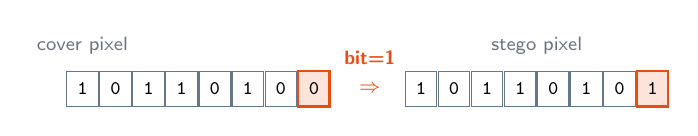
\begin{tikzpicture}[node distance=0.06cm]
% cover byte
\node[font=\scriptsize\color{umgray}] (lblc) at (0,0.55) {cover pixel};
\node[bitcell] (b7) at (0   ,0)   {1};
\node[bitcell] (b6) at (0.42,0)   {0};
\node[bitcell] (b5) at (0.84,0)   {1};
\node[bitcell] (b4) at (1.26,0)   {1};
\node[bitcell] (b3) at (1.68,0)   {0};
\node[bitcell] (b2) at (2.10,0)   {1};
\node[bitcell] (b1) at (2.52,0)   {0};
\node[bitlsb]  (b0) at (2.94,0)   {0};

% arrow + payload bit
\node[font=\scriptsize\color{umorange}\bfseries] at (3.65,0.0) {$\Rightarrow$};
\node[font=\scriptsize\color{umorange}\bfseries] at (3.65,0.4) {bit=1};

% stego byte
\node[bitcell] at (4.30,0) {1};
\node[bitcell] at (4.72,0) {0};
\node[bitcell] at (5.14,0) {1};
\node[bitcell] at (5.56,0) {1};
\node[bitcell] at (5.98,0) {0};
\node[bitcell] at (6.40,0) {1};
\node[bitcell] at (6.82,0) {0};
\node[bitlsb]  at (7.24,0) {1};
\node[font=\scriptsize\color{umgray}] at (5.77,0.55) {stego pixel};
\end{tikzpicture}
\end{center}
\vspace{-0.1cm}
{\scriptsize\color{umgray}One pixel \textendash\ one payload bit. Detected by RS, $\chi^2$, Sample Pairs.}
\end{column}
\begin{column}{0.49\textwidth}
\begin{block}{Frequency: DCT-LSB (JSteg-style)}
Flip the LSB of \emph{non-zero} quantised AC coefficients in each $8\!\times\!8$ block. Skip DC and $|c|\!=\!1$ (Westfeld-pair stable). JPEG Q=95.
\end{block}
\vspace{-0.05cm}
\begin{center}
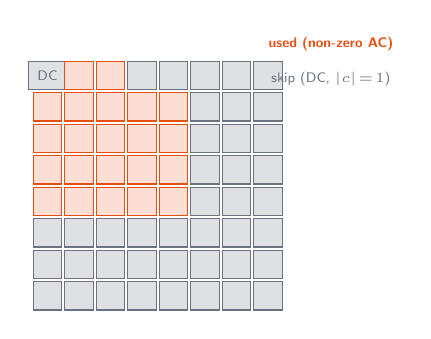
\begin{tikzpicture}
% 8x8 DCT block: corner = DC (skip, grey), some |c|=1 cells grey, others orange
\foreach \r in {0,...,7} {
  \foreach \c in {0,...,7} {
    \pgfmathsetmacro{\xx}{0.40*\c}
    \pgfmathsetmacro{\yy}{-0.40*\r}
    % skip top-left (DC) and a band of unity-magnitude coefficients (mid-high frequency)
    \ifnum\r=0
      \ifnum\c=0
        \node[dctskip] at (\xx,\yy) {DC};
      \else
        \ifnum\c<3 \node[dctused] at (\xx,\yy) {}; \else \node[dctskip] at (\xx,\yy) {}; \fi
      \fi
    \else
      \pgfmathsetmacro{\rr}{\r+\c}
      \ifnum\r>4 \node[dctskip] at (\xx,\yy) {}; \else
        \ifnum\c>4 \node[dctskip] at (\xx,\yy) {}; \else
          \node[dctused] at (\xx,\yy) {};
        \fi
      \fi
    \fi
  }
}
% Legend
\node[font=\tiny\color{umorange}\bfseries] at (3.6, 0.40) {used (non-zero AC)};
\node[font=\tiny\color{umgray}]            at (3.6,-0.05) {skip (DC, $|c|\!=\!1$)};
\end{tikzpicture}
\end{center}
\vspace{-0.1cm}
{\scriptsize\color{umgray}Detected by $\chi^2$-DCT and Calibration $\chi^2$.}
\end{column}
\end{columns}
\end{frame}

% ============================================================
% 7. Detector Choices and Mechanisms (NEW: chi^2 PoV histogram)
% ============================================================
\begin{frame}{Detector Mechanisms}
\footnotesize
\begin{columns}[T]
\begin{column}{0.46\textwidth}
\begin{block}{Pairs-of-Values intuition}
$\chi^2$ tests the prediction that LSB embedding equalises the counts of value pairs $\{2k, 2k\!+\!1\}$. Bars within each pair converge in stego images.
\end{block}
\vspace{0.05cm}
\begin{center}
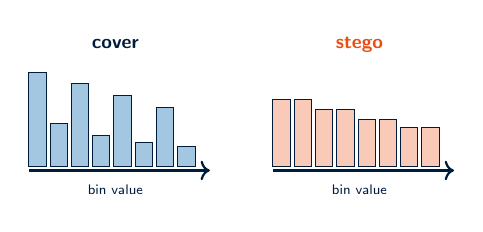
\begin{tikzpicture}[
  bar/.style={draw=umdark, fill=umlight!50, line width=0.3pt},
  barb/.style={draw=umdark, fill=umlight, line width=0.3pt},
  barflat/.style={draw=umdark, fill=umorange!30, line width=0.3pt},
  axisstyle/.style={->, thick, umdark}
]
% Cover histogram (uneven pairs)
\begin{scope}[shift={(0,0)}]
\foreach \i/\h in {0/1.20, 1/0.55, 2/1.05, 3/0.40, 4/0.90, 5/0.30, 6/0.75, 7/0.25} {
  \pgfmathsetmacro{\xx}{0.27*\i}
  \draw[bar] (\xx,0) rectangle (\xx+0.22,\h);
}
\draw[axisstyle] (0,-0.05) -- (2.30,-0.05);
\node[font=\tiny\color{umdark}] at (1.10,-0.30) {bin value};
\node[font=\scriptsize\bfseries\color{umdark}] at (1.10,1.55) {cover};
\end{scope}
% Stego histogram (pairs flattened)
\begin{scope}[shift={(3.10,0)}]
\foreach \i/\h in {0/0.85, 1/0.85, 2/0.72, 3/0.72, 4/0.60, 5/0.60, 6/0.50, 7/0.50} {
  \pgfmathsetmacro{\xx}{0.27*\i}
  \draw[barflat] (\xx,0) rectangle (\xx+0.22,\h);
}
\draw[axisstyle] (0,-0.05) -- (2.30,-0.05);
\node[font=\tiny\color{umdark}] at (1.10,-0.30) {bin value};
\node[font=\scriptsize\bfseries\color{umorange}] at (1.10,1.55) {stego};
\end{scope}
\end{tikzpicture}
\end{center}
\vspace{-0.05cm}
{\scriptsize\color{umgray}$\chi^2$ score rises whenever paired bars are mismatched in the cover and equalise in the stego.}
\end{column}
\begin{column}{0.50\textwidth}
\begin{block}{Spatial}
\begin{itemize}\setlength{\itemsep}{1pt}
\item \textbf{RS} \icite{(Fridrich 2001):} regular/singular pixel-group ratios
\item \textbf{$\chi^2$} \icite{(Westfeld 1999):} PoV (left)
\item \textbf{Sample Pairs} \icite{(Dumitrescu 2003):} traces on adjacent-pixel multisets
\end{itemize}
\end{block}
\begin{block}{Frequency}
\begin{itemize}\setlength{\itemsep}{1pt}
\item \textbf{$\chi^2$-DCT} \icite{(Westfeld 1999):} PoV on AC coefficients
\item \textbf{Calibration $\chi^2$} \icite{(Fridrich 2003):} non-block-aligned crop + recompress reference
\end{itemize}
\end{block}
\end{column}
\end{columns}
\vspace{0.05cm}
{\tiny\color{umgray}\textbf{Why training-free:} no learned parameters $\Rightarrow$ AUC differences reflect carrier statistics, not training-set mismatch.}
\end{frame}

% ============================================================
% 8. Pipeline Structure  (NEW: 5-stage flow diagram)
% ============================================================
\section{Pipeline Structure}
\begin{frame}{Pipeline Structure}
\small
\begin{center}
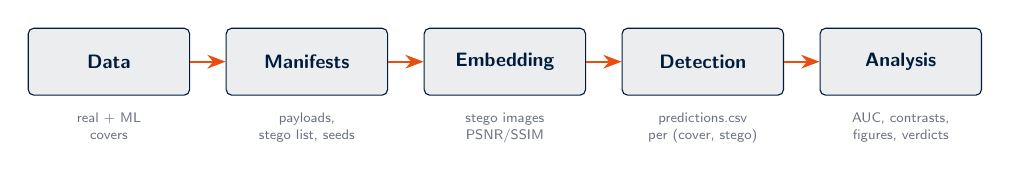
\begin{tikzpicture}[node distance=0.45cm]
\node[pstage] (data) {Data};
\node[pstage, right=of data] (man)  {Manifests};
\node[pstage, right=of man]  (emb)  {Embedding};
\node[pstage, right=of emb]  (det)  {Detection};
\node[pstage, right=of det]  (agg)  {Analysis};

\draw[parrow] (data) -- (man);
\draw[parrow] (man)  -- (emb);
\draw[parrow] (emb)  -- (det);
\draw[parrow] (det)  -- (agg);

\node[pout, below=0.10cm of data] {real + ML\\covers};
\node[pout, below=0.10cm of man]  {payloads,\\stego list, seeds};
\node[pout, below=0.10cm of emb]  {stego images\\PSNR/SSIM};
\node[pout, below=0.10cm of det]  {predictions.csv\\per (cover, stego)};
\node[pout, below=0.10cm of agg]  {AUC, contrasts,\\figures, verdicts};
\end{tikzpicture}
\end{center}
\vspace{0.1cm}
\begin{columns}[T]
\begin{column}{0.49\textwidth}
\begin{block}{Five sequential stages}
\begin{itemize}
\item Data and manifests are reproducible from seeds.
\item Embedding writes one stego file per condition.
\item Detection scores cover+stego pairs.
\item Aggregation derives all RQ outputs.
\end{itemize}
\end{block}
\end{column}
\begin{column}{0.49\textwidth}
\begin{block}{Run isolation}
\begin{itemize}
\item Each run lives in \texttt{runs/<id>/}.
\item Config frozen in \texttt{config.json}.
\item Re-runs are idempotent: done work is skipped.
\end{itemize}
\end{block}
\end{column}
\end{columns}
\end{frame}

% ============================================================
% 9. Web Platform
% ============================================================
\section{Web Platform}
\begin{frame}{Web Platform and Live Monitoring}
\small
\begin{columns}[T]
\begin{column}{0.49\textwidth}
\begin{block}{Architecture}
\begin{itemize}
\item Local Python HTTP server (stdlib only)
\item Single-page browser client, no build step
\item Endpoints: list / launch / preview / kill / detail
\item Launch spawns the runner as a subprocess
\end{itemize}
\end{block}
\end{column}
\begin{column}{0.49\textwidth}
\begin{block}{Live observability}
\begin{itemize}
\item Subprocess stdout via Server-Sent Events
\item Browser terminal panel shows progress live
\item Preview validates config before any compute
\item Run-detail surfaces metrics, figures, gallery
\end{itemize}
\end{block}
\end{column}
\end{columns}
\vspace{0.05cm}
{\scriptsize\color{umgray}Power estimate in the drawer: Hanley--McNeil computed live in JavaScript, colour-coded against the proposal threshold $\delta\!=\!0.05$.}
\end{frame}

% ============================================================
% 10. Statistical Analysis  (NEW: paired DeLong sketch)
% ============================================================
\section{Statistical Analysis}
\begin{frame}{Statistical Analysis}
\footnotesize
\begin{columns}[T]
\begin{column}{0.50\textwidth}
\begin{block}{Tests}
\begin{itemize}\setlength{\itemsep}{1pt}
\item DeLong paired ROC test for correlated AUCs \icite{(DeLong 1988)}
\item Bonferroni--Holm correction (confirmatory); 95\% CIs (exploratory)
\item Equivalence margin $\pm 0.025$ AUC for RQ5
\end{itemize}
\end{block}
\begin{block}{Power (Hanley--McNeil)}
\begin{itemize}\setlength{\itemsep}{1pt}
\item $\alpha = 0.05$, target power $0.80$; family size 15 strata per RQ
\item Min detectable $\delta_\text{AUC}$ at $N\!=\!1{,}000$ well below the $\delta_\text{min}\!=\!0.05$ proposal threshold; $N\!=\!3{,}000$ tightens every CI by $\sqrt{3}\!\approx\!1.73\times$
\end{itemize}
\end{block}
\end{column}
\begin{column}{0.46\textwidth}
\begin{center}
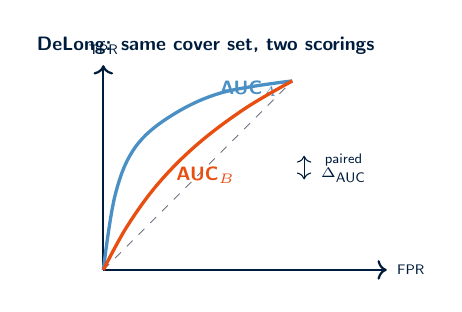
\begin{tikzpicture}[
  axarrow/.style={->, thick, umdark},
  rocA/.style={very thick, umlight},
  rocB/.style={very thick, umorange},
  diag/.style={dashed, umgray, line width=0.3pt}
]
% axes
\draw[axarrow] (0,0) -- (3.6,0)  node[right, font=\tiny\color{umgray}] {FPR};
\draw[axarrow] (0,0) -- (0,2.6)  node[above, font=\tiny\color{umgray}] {TPR};
\draw[diag] (0,0) -- (2.4,2.4);
% Curve A: high AUC
\draw[rocA] plot[smooth, tension=0.6] coordinates {(0,0) (0.15,0.95) (0.4,1.55) (0.85,1.95) (1.5,2.25) (2.4,2.4)};
\node[font=\scriptsize\color{umlight}\bfseries] at (1.85,2.30) {AUC$_A$};
% Curve B: lower AUC (different carrier)
\draw[rocB] plot[smooth, tension=0.6] coordinates {(0,0) (0.30,0.55) (0.7,1.10) (1.20,1.60) (1.80,2.05) (2.4,2.4)};
\node[font=\scriptsize\color{umorange}\bfseries] at (1.30,1.20) {AUC$_B$};
% Delta label
\node[font=\tiny\color{umdark}] at (3.05,1.40) {paired};
\node[font=\tiny\color{umdark}] at (3.05,1.20) {$\Delta_\text{AUC}$};
\draw[<->, umdark] (2.55,1.15) -- (2.55,1.45);
% Title
\node[font=\scriptsize\bfseries\color{umdark}] at (1.30,2.85) {DeLong: same cover set, two scorings};
\end{tikzpicture}
\end{center}
\vspace{0.05cm}
{\scriptsize\color{umgray}Each $\Delta_\text{AUC}$ comes from a single stratum; Holm controls the family-wise error rate across 15 strata.}
\end{column}
\end{columns}
\end{frame}

% ============================================================
% 10b. Reproducibility / run-artefact claim (precedes Results)
% ============================================================
\begin{frame}{Run Artefacts and Reproducibility}
\scriptsize
\begin{columns}[T]
\begin{column}{0.49\textwidth}
\begin{block}{What the 3{,}000-group run produced}
\centering\renewcommand{\arraystretch}{1.05}
\begin{tabular}{l@{\hskip 6pt}r}
\textbf{Artefact} & \textbf{Count} \\
\midrule
Cover images (real + ML-A + ML-B) & 18{,}000 \\
Stego images (3 sources $\times$ 12 conds) & 108{,}000 \\
Detector predictions (6 detectors) & 648{,}000 \\
Aggregated metrics CSVs & 19 \\
Figures (ROC panels, contrasts, forest) & 61 \\
RQ verdicts (JSON + Markdown) & 2 \\
\midrule
On-disk artefacts & $\sim$13.5 GB \\
Wall-clock (cover prep + embedding + analysis) & $\sim$13 h \\
\end{tabular}
\end{block}
\end{column}
\begin{column}{0.49\textwidth}
\begin{block}{Reproducibility guarantees}
\begin{itemize}\setlength{\itemsep}{1pt}
\item \textbf{Seeded} every stage: split, payload, embedding, ML generation. Re-running yields bit-identical covers / payloads / stego (within engine determinism).
\item \textbf{Frozen config}: each run writes \texttt{config.json} with every parameter -- active detectors, payload fill rates, seeds.
\item \textbf{Manifest-driven}: every condition recorded in CSV manifests before execution.
\item \textbf{Idempotent}: re-runs skip work already on disk; partial failures resume cleanly.
\item \textbf{245 automated tests} cover detectors, embedders, RQ verdict logic, analysis pipeline.
\item \textbf{Open source}: all code + figures derivable from \texttt{predictions.csv}.
\end{itemize}
\end{block}
\end{column}
\end{columns}
\end{frame}

% ============================================================
% 10c. Stego image quality
% ============================================================
\begin{frame}{Stego Image Quality (PSNR / SSIM)}
\scriptsize
\begin{columns}[T]
\begin{column}{0.40\textwidth}
\begin{block}{Why we track this}
\begin{itemize}\setlength{\itemsep}{1pt}
\item PSNR and SSIM (Wang 2004) measure how much the stego image deviates from its cover.
\item PSNR\,$\gtrsim$\,40 dB and SSIM\,$\gtrsim$\,0.99 are the standard ``visually imperceptible'' floor.
\item Confirms the carrier-source effect we report is \emph{not} a perceptual-distortion artefact.
\end{itemize}
\end{block}
\begin{exampleblock}{Per-source equivalence}
SSIM\,$\geq\!0.999$ everywhere. PSNR is similar across real (58.2), ml\_a (59.2), ml\_b (59.2 dB) -- detectability differences happen at the same distortion budget.
\end{exampleblock}
\end{column}
\begin{column}{0.56\textwidth}
\begin{center}
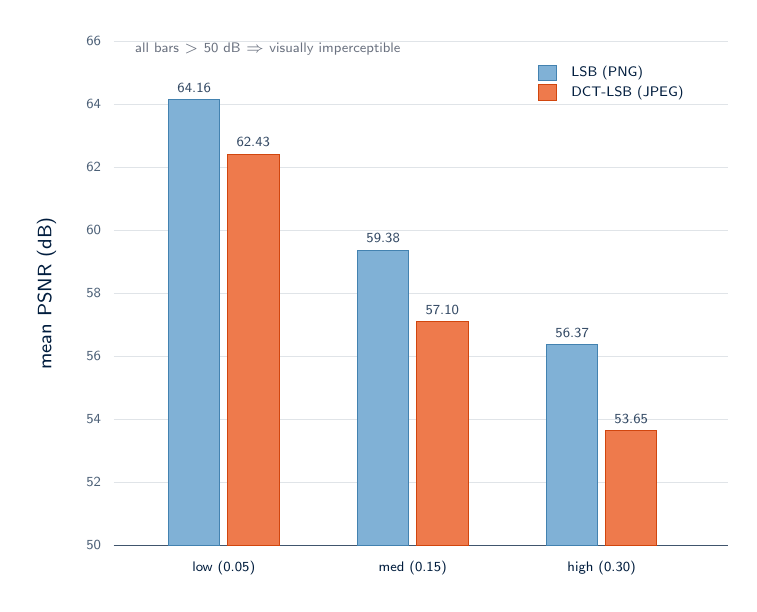
\begin{tikzpicture}[
  barlsb/.style={draw=umlight!90!black, fill=umlight!70, line width=0.25pt},
  bardct/.style={draw=umorange!90!black, fill=umorange!75, line width=0.25pt},
]
% y: PSNR from 50 to 66 dB → 0..6.4 cm (multiplier 0.4)
\foreach \v in {50,52,54,56,58,60,62,64,66} {
  \pgfmathsetmacro{\y}{(\v - 50) * 0.4}
  \draw[umdark!12, line width=0.3pt] (0,\y) -- (7.8,\y);
  \node[font=\tiny\color{umdark!70}, left=1pt] at (0,\y) {\v};
}
\draw[umdark!75, line width=0.5pt] (0,0) -- (7.8,0);
\node[font=\scriptsize\color{umdark}, rotate=90] at (-0.85, 3.2) {mean PSNR (dB)};
% Highlight 40 dB "imperceptible" line is below our axis range; instead label "all > 50 dB"
\node[font=\tiny\color{umgray}, anchor=west] at (0.15, 6.3) {all bars $>$ 50 dB $\Rightarrow$ visually imperceptible};

\def\bw{0.65}
\def\bg{0.10}
\foreach \i/\pl/\lsb/\dct in {
  0/{low (0.05)}/64.16/62.43,
  1/{med (0.15)}/59.38/57.10,
  2/{high (0.30)}/56.37/53.65
} {
  \pgfmathsetmacro{\xc}{1.4 + \i*2.4}
  \pgfmathsetmacro{\xa}{\xc - 0.5*\bw - \bg/2}
  \pgfmathsetmacro{\xb}{\xc + 0.5*\bw + \bg/2}
  \pgfmathsetmacro{\hlsb}{(\lsb - 50) * 0.4}
  \pgfmathsetmacro{\hdct}{(\dct - 50) * 0.4}
  \draw[barlsb] (\xa-\bw/2,0) rectangle (\xa+\bw/2,\hlsb);
  \draw[bardct] (\xb-\bw/2,0) rectangle (\xb+\bw/2,\hdct);
  \node[font=\tiny\color{umdark!80}, above=-1pt] at (\xa,\hlsb) {\lsb};
  \node[font=\tiny\color{umdark!80}, above=-1pt] at (\xb,\hdct) {\dct};
  \node[font=\tiny\color{umdark}, below=2pt] at (\xc,0) {\pl};
}
% legend
\begin{scope}[shift={(5.40, 5.6)}]
  \draw[barlsb] (0,0.30) rectangle (0.22,0.50);
  \draw[bardct] (0,0.05) rectangle (0.22,0.25);
  \node[font=\tiny\color{umdark}, right=2pt] at (0.22,0.40) {LSB (PNG)};
  \node[font=\tiny\color{umdark}, right=2pt] at (0.22,0.15) {DCT-LSB (JPEG)};
\end{scope}
\end{tikzpicture}

\end{center}
\end{column}
\end{columns}
\end{frame}

% ============================================================
% 11. Results: per-detector overview
% ============================================================
\section{Results}
\begin{frame}{Headline -- AUC by Carrier Source and Detector}
\footnotesize
\begin{center}
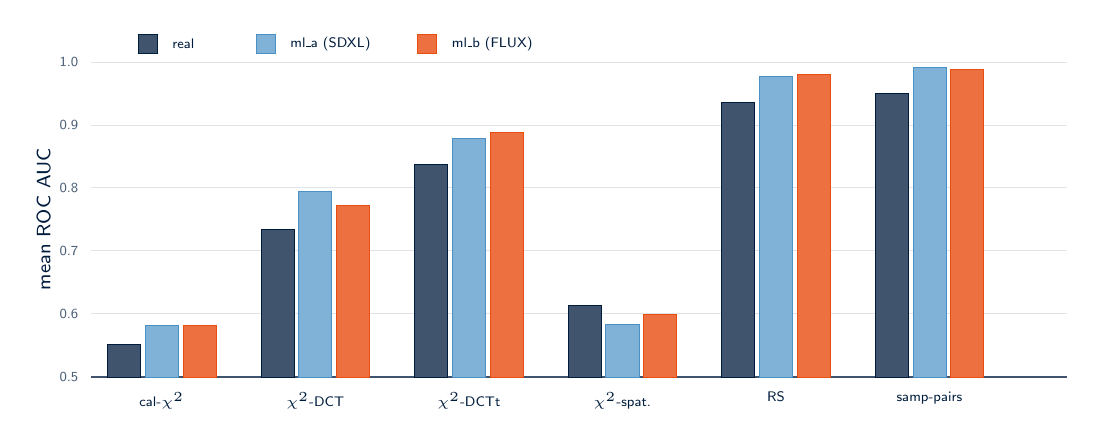
\begin{tikzpicture}[
  barlabel/.style={font=\tiny\color{umdark!70}},
  bargrey/.style={draw=umdark, fill=umdark!75, line width=0.25pt},
  barblue/.style={draw=umlight, fill=umlight!70, line width=0.25pt},
  baroran/.style={draw=umorange, fill=umorange!80, line width=0.25pt},
]
% y-axis gridlines + labels (AUC 0.5..1.0 mapped to 0..5 cm)
\foreach \v in {0.5,0.6,0.7,0.8,0.9,1.0} {
  \pgfmathsetmacro{\y}{(\v - 0.5) * 8}
  \draw[umdark!12, line width=0.3pt] (0,\y) -- (12.4,\y);
  \node[font=\tiny\color{umdark!70}, left=1pt] at (0,\y) {\v};
}
\draw[umdark!75, line width=0.5pt] (0,0) -- (12.4,0);
\node[font=\scriptsize\color{umdark}, rotate=90] at (-0.6,2.0) {mean ROC AUC};

\def\bw{0.42}
\def\bg{0.06}
\foreach \i/\name/\real/\mla/\mlb in {
  0/{cal-$\chi^2$}/0.552/0.582/0.582,
  1/{$\chi^2$-DCT}/0.734/0.795/0.772,
  2/{$\chi^2$-DCTt}/0.838/0.879/0.888,
  3/{$\chi^2$-spat.}/0.614/0.583/0.599,
  4/{RS}/0.936/0.977/0.981,
  5/{samp-pairs}/0.950/0.991/0.988
} {
  \pgfmathsetmacro{\xc}{0.9 + \i*1.95}
  \pgfmathsetmacro{\xa}{\xc - 1.5*\bw - \bg}
  \pgfmathsetmacro{\xb}{\xc - 0.5*\bw}
  \pgfmathsetmacro{\xcc}{\xc + 0.5*\bw + \bg}
  \pgfmathsetmacro{\hreal}{(\real - 0.5) * 8}
  \pgfmathsetmacro{\hmla}{(\mla - 0.5) * 8}
  \pgfmathsetmacro{\hmlb}{(\mlb - 0.5) * 8}
  \draw[bargrey] (\xa,0)  rectangle (\xa+\bw,\hreal);
  \draw[barblue] (\xb,0)  rectangle (\xb+\bw,\hmla);
  \draw[baroran] (\xcc,0) rectangle (\xcc+\bw,\hmlb);
  \node[font=\tiny\color{umdark}, below=2pt] at (\xc,0) {\name};
}

% Legend positioned at top of chart (well clear of any bars)
\begin{scope}[shift={(0.6, 4.05)}]
  \draw[bargrey] (0,0.06) rectangle (0.24,0.30);
  \node[font=\tiny\color{umdark}, right=2pt] at (0.24,0.18) {real};
  \draw[barblue] (1.50,0.06) rectangle (1.74,0.30);
  \node[font=\tiny\color{umdark}, right=2pt] at (1.74,0.18) {ml\_a (SDXL)};
  \draw[baroran] (3.55,0.06) rectangle (3.79,0.30);
  \node[font=\tiny\color{umdark}, right=2pt] at (3.79,0.18) {ml\_b (FLUX)};
\end{scope}
\end{tikzpicture}
\end{center}
\vspace{-0.05cm}
\begin{exampleblock}{Carrier source matters, direction depends on the detector}
Five of six detectors find ML carriers \emph{easier} to attack (orange/blue $>$ dark for cal-$\chi^2$, $\chi^2$-DCT, $\chi^2$-DCT-tiled, RS, sample-pairs). \textbf{$\chi^2$-spatial} is the lone hold-out -- on LSB the diffusion outputs are \emph{harder} to detect, a sign flip the supplementary pAUC view dissolves.
\end{exampleblock}
\end{frame}

% ============================================================
% 12. Results: RQ1
% ============================================================
\begin{frame}{RQ1 -- Real vs.\ Pooled ML}
\scriptsize
\begin{columns}[T]
\begin{column}{0.46\textwidth}
\begin{block}{Test}
Paired DeLong per stratum (detector $\times$ method $\times$ payload), Holm-adjusted across 18 strata (6 detectors $\times$ 3 payload levels).
\end{block}
\begin{block}{Headline finding ($N\!=\!3{,}000$)}
\begin{itemize}\setlength{\itemsep}{1pt}
\item Pooled $\Delta_\text{AUC}$: $\boldsymbol{-0.0129}$ \\[1pt] (95\% CI $[-0.0137, -0.0121]$)
\item Significant after Holm: \textbf{16 / 18} (+2, $-$14)
\item Practically relevant ($|\Delta|\!\geq\!0.05$): \textbf{4 / 16} \\ (all ML $>$ real; 12 trivial)
\item Verdict: \textbf{mixed} -- direction-consistent at the practical-significance gate, all ML $>$ real
\end{itemize}
\end{block}
\end{column}
\begin{column}{0.50\textwidth}
\begin{center}
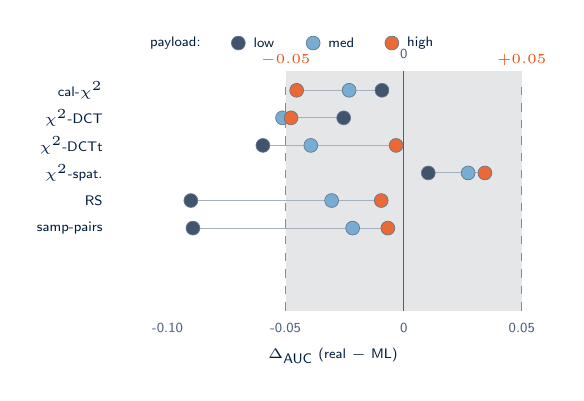
\begin{tikzpicture}[
  detrow/.style={font=\tiny\color{umdark}},
  dotlow/.style={circle, draw=umdark!60, fill=umdark!75,   inner sep=0pt, minimum size=5pt, line width=0.25pt},
  dotmed/.style={circle, draw=umdark!60, fill=umlight!75,  inner sep=0pt, minimum size=5pt, line width=0.25pt},
  dothigh/.style={circle, draw=umdark!60, fill=umorange!85, inner sep=0pt, minimum size=5pt, line width=0.25pt},
]
% x mapping: Δ ∈ [-0.12, +0.06] → [0, 5.4] cm (multiplier 30).
% Zero at x=3.6; ±0.05 at 2.1/5.1. Compressed to fit the 0.50-textwidth column.
\fill[umgray!18] (2.1,-2.85) rectangle (5.1,0.20);
\draw[umdark!70, line width=0.4pt] (3.6,-2.85) -- (3.6,0.20);
\node[font=\tiny\color{umdark!70}, above=1pt] at (3.6,0.20) {0};
\draw[umorange!85, line width=0.4pt, dashed] (2.1,-2.85) -- (2.1,0.10);
\draw[umorange!85, line width=0.4pt, dashed] (5.1,-2.85) -- (5.1,0.10);
\node[font=\tiny\color{umorange}, above=1pt] at (2.1,0.10) {$-0.05$};
\node[font=\tiny\color{umorange}, above=1pt] at (5.1,0.10) {$+0.05$};
\foreach \v in {-0.10,-0.05,0,0.05} {
  \pgfmathsetmacro{\x}{(\v + 0.12) * 30}
  \node[font=\tiny\color{umdark!70}, below=1pt] at (\x,-2.85) {\v};
}
\node[font=\tiny\color{umdark}, below=10pt] at (2.7,-2.85) {$\Delta_\text{AUC}$ (real $-$ ML)};

\foreach \i/\labl/\dl/\dm/\dh in {
  0/{cal-$\chi^2$}/-0.0092/-0.0231/-0.0453,
  1/{$\chi^2$-DCT}/-0.0254/-0.0513/-0.0477,
  2/{$\chi^2$-DCTt}/-0.0596/-0.0393/-0.0032,
  3/{$\chi^2$-spat.}/0.0104/0.0273/0.0344,
  4/{RS}/-0.0901/-0.0305/-0.0095,
  5/{samp-pairs}/-0.0892/-0.0216/-0.0067
} {
  \pgfmathsetmacro{\y}{-\i*0.35 - 0.05}
  \node[detrow, anchor=east] at (-0.10,\y) {\labl};
  \pgfmathsetmacro{\xa}{(\dl + 0.12) * 30}
  \pgfmathsetmacro{\xb}{(\dm + 0.12) * 30}
  \pgfmathsetmacro{\xcc}{(\dh + 0.12) * 30}
  \draw[umdark!35, line width=0.35pt] (\xa,\y) -- (\xcc,\y);
  \node[dotlow]  at (\xa,\y) {};
  \node[dotmed]  at (\xb,\y) {};
  \node[dothigh] at (\xcc,\y) {};
}
% legend (above the plot, inside; fit within 0..5.4 horizontal range)
\node[font=\tiny\color{umdark}] at (0.7,0.55) {payload:};
\node[dotlow]  at (1.5,0.55) {};
\node[font=\tiny\color{umdark}, right=2pt] at (1.5,0.55) {low};
\node[dotmed]  at (2.45,0.55) {};
\node[font=\tiny\color{umdark}, right=2pt] at (2.45,0.55) {med};
\node[dothigh] at (3.45,0.55) {};
\node[font=\tiny\color{umdark}, right=2pt] at (3.45,0.55) {high};
\end{tikzpicture}
\end{center}
\vspace{-0.05cm}
{\scriptsize\color{umgray}Each detector row spans its 3 payload strata. Grey band = trivial zone $|\Delta|\!<\!0.05$. \textbf{Four} dots clear the practical-significance threshold, all on the ML-easier side; $\chi^2$-spatial sits opposite.}
\end{column}
\end{columns}
\end{frame}

% ============================================================
% 12b. Results: RQ1 -- per-stratum scatter
% ============================================================
\begin{frame}{RQ1 -- Per-Stratum AUC (real vs.\ pooled ML)}
\scriptsize
\begin{columns}[T]
\begin{column}{0.42\textwidth}
\begin{block}{Reading the plot}
\begin{itemize}\setlength{\itemsep}{1pt}
\item Each dot = one stratum (6 detectors $\times$ 3 payload levels = 18).
\item \textbf{Shape} = detector; \textbf{fill colour} = payload.
\item Above the diagonal $\Rightarrow$ ML easier to detect;
   below $\Rightarrow$ real easier.
\item Orange band = $\pm 0.05$ practical margin.
\end{itemize}
\end{block}
\begin{exampleblock}{What to look for}
\begin{itemize}\setlength{\itemsep}{1pt}
\item All three \emph{triangles} ($\chi^2$-spat.) lie below the diagonal -- the lone real-easier outlier.
\item The four dots outside the orange band on the ML-easier side: RS\,low, samp-pairs\,low, $\chi^2$-DCTt\,low, $\chi^2$-DCT\,med -- four independent detector families agreeing.
\end{itemize}
\end{exampleblock}
\end{column}
\begin{column}{0.54\textwidth}
\begin{center}
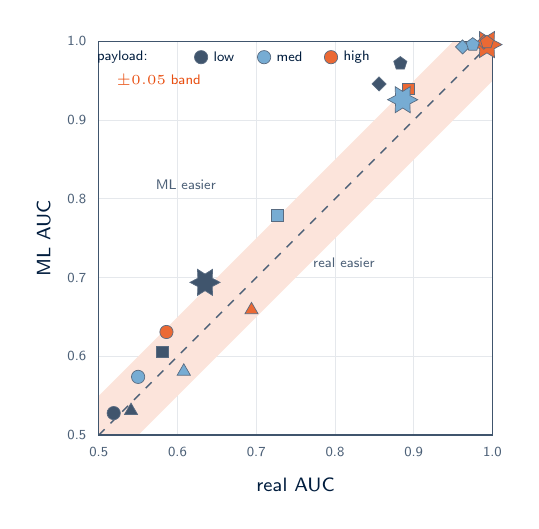
\begin{tikzpicture}[
  mCircle/.style ={circle, draw=umdark!65, inner sep=0pt, minimum size=4.8pt, line width=0.25pt},
  mSquare/.style ={rectangle, draw=umdark!65, inner sep=0pt, minimum size=4.2pt, line width=0.25pt},
  mDiamond/.style={diamond, draw=umdark!65, inner sep=0pt, minimum width=5.2pt, minimum height=5.2pt, line width=0.25pt},
  mTri/.style    ={regular polygon, regular polygon sides=3, draw=umdark!65, inner sep=0pt, minimum size=5.5pt, line width=0.25pt},
  mPenta/.style  ={regular polygon, regular polygon sides=5, draw=umdark!65, inner sep=0pt, minimum size=5pt, line width=0.25pt},
  mStar/.style   ={star, star points=6, star point ratio=0.55, draw=umdark!65, inner sep=0pt, minimum size=6.0pt, line width=0.25pt},
]
% AUC range [0.5, 1.0] mapped to [0, 5] cm.
\def\sz{5}
\foreach \v in {0.5,0.6,0.7,0.8,0.9,1.0} {
  \pgfmathsetmacro{\xy}{(\v - 0.5) * 10}
  \draw[umdark!10, line width=0.3pt] (0,\xy) -- (\sz,\xy);
  \draw[umdark!10, line width=0.3pt] (\xy,0) -- (\xy,\sz);
  \node[font=\tiny\color{umdark!70}, left=1pt] at (0,\xy) {\v};
  \node[font=\tiny\color{umdark!70}, below=1pt] at (\xy,0) {\v};
}
\fill[umorange!15] (0,0.5) -- (4.5,5) -- (5,5) -- (5,4.5) -- (0.5,0) -- (0,0) -- cycle;
\draw[umdark!70, line width=0.5pt, dashed] (0,0) -- (\sz,\sz);
\draw[umdark!75, line width=0.5pt] (0,0) rectangle (\sz,\sz);
\node[font=\scriptsize\color{umdark}, below=12pt] at (\sz/2, 0) {real AUC};
\node[font=\scriptsize\color{umdark}, rotate=90] at (-0.7, \sz/2) {ML AUC};

\node[font=\tiny\color{umdark!70}, anchor=south west] at (2.6,2.0) {real easier};
\node[font=\tiny\color{umdark!70}, anchor=south west] at (0.6,3.0) {ML easier};
\node[font=\tiny\color{umorange}, anchor=south west] at (0.10,4.30) {$\pm 0.05$ band};

% 18 dots: shape encodes detector, fill encodes payload (umdark=low, umlight=med, umorange=high)
% cal-χ² (circle)
\node[mCircle, fill=umdark!75]  at ({(0.519-0.5)*10},{(0.528-0.5)*10}) {};
\node[mCircle, fill=umlight!75] at ({(0.550-0.5)*10},{(0.574-0.5)*10}) {};
\node[mCircle, fill=umorange!85] at ({(0.586-0.5)*10},{(0.631-0.5)*10}) {};
% χ²-DCT (square)
\node[mSquare, fill=umdark!75]  at ({(0.581-0.5)*10},{(0.606-0.5)*10}) {};
\node[mSquare, fill=umlight!75] at ({(0.727-0.5)*10},{(0.779-0.5)*10}) {};
\node[mSquare, fill=umorange!85] at ({(0.893-0.5)*10},{(0.940-0.5)*10}) {};
% χ²-DCT-tiled (star)
\node[mStar, fill=umdark!75]   at ({(0.635-0.5)*10},{(0.694-0.5)*10}) {};
\node[mStar, fill=umlight!75]  at ({(0.886-0.5)*10},{(0.926-0.5)*10}) {};
\node[mStar, fill=umorange!85] at ({(0.993-0.5)*10},{(0.996-0.5)*10}) {};
% χ²-spatial (triangle) -- the sign-flip outlier, below the diagonal
\node[mTri, fill=umdark!75]   at ({(0.541-0.5)*10},{(0.531-0.5)*10}) {};
\node[mTri, fill=umlight!75]  at ({(0.608-0.5)*10},{(0.581-0.5)*10}) {};
\node[mTri, fill=umorange!85] at ({(0.694-0.5)*10},{(0.659-0.5)*10}) {};
% RS (diamond)
\node[mDiamond, fill=umdark!75]  at ({(0.856-0.5)*10},{(0.946-0.5)*10}) {};
\node[mDiamond, fill=umlight!75] at ({(0.962-0.5)*10},{(0.993-0.5)*10}) {};
\node[mDiamond, fill=umorange!85] at ({(0.989-0.5)*10},{(0.999-0.5)*10}) {};
% sample-pairs (pentagon)
\node[mPenta, fill=umdark!75]  at ({(0.883-0.5)*10},{(0.972-0.5)*10}) {};
\node[mPenta, fill=umlight!75] at ({(0.975-0.5)*10},{(0.996-0.5)*10}) {};
\node[mPenta, fill=umorange!85] at ({(0.993-0.5)*10},{(0.999-0.5)*10}) {};

% Payload legend (colors) -- top of plot
\node[font=\tiny\color{umdark}] at (0.30,4.80) {payload:};
\node[mCircle, fill=umdark!75]  at (1.30,4.80) {};
\node[font=\tiny\color{umdark}, right=1pt] at (1.30,4.80) {low};
\node[mCircle, fill=umlight!75] at (2.10,4.80) {};
\node[font=\tiny\color{umdark}, right=1pt] at (2.10,4.80) {med};
\node[mCircle, fill=umorange!85] at (2.95,4.80) {};
\node[font=\tiny\color{umdark}, right=1pt] at (2.95,4.80) {high};
\end{tikzpicture}

\vspace{0.05cm}
{\tiny\color{umdark}\textbf{detectors}\hspace{0.2em}
 \tikz[baseline=-2pt]\node[circle, draw=umdark!65, fill=umdark!30, inner sep=0pt, minimum size=4.5pt, line width=0.25pt]{};\,cal-$\chi^2$\hspace{0.5em}
 \tikz[baseline=-2pt]\node[rectangle, draw=umdark!65, fill=umdark!30, inner sep=0pt, minimum size=3.8pt, line width=0.25pt]{};\,$\chi^2$-DCT\hspace{0.5em}
 \tikz[baseline=-2pt]\node[star, star points=6, star point ratio=0.55, draw=umdark!65, fill=umdark!30, inner sep=0pt, minimum size=5pt, line width=0.25pt]{};\,$\chi^2$-DCTt\hspace{0.5em}
 \tikz[baseline=-2pt]\node[regular polygon, regular polygon sides=3, draw=umdark!65, fill=umdark!30, inner sep=0pt, minimum size=5pt, line width=0.25pt]{};\,$\chi^2$-spat.\hspace{0.5em}
 \tikz[baseline=-2pt]\node[diamond, draw=umdark!65, fill=umdark!30, inner sep=0pt, minimum width=4.8pt, minimum height=4.8pt, line width=0.25pt]{};\,RS\hspace{0.5em}
 \tikz[baseline=-2pt]\node[regular polygon, regular polygon sides=5, draw=umdark!65, fill=umdark!30, inner sep=0pt, minimum size=4.5pt, line width=0.25pt]{};\,samp-pairs}
\end{center}
\end{column}
\end{columns}
\end{frame}

% ============================================================
% 13. Results: RQ2
% ============================================================
\begin{frame}{RQ2 -- SDXL vs.\ FLUX within ML}
\scriptsize
\begin{columns}[T]
\begin{column}{0.46\textwidth}
\begin{block}{Test}
Paired DeLong on caption-matched SDXL/FLUX pairs, Holm-adjusted across 18 strata.
\end{block}
\begin{block}{Headline finding ($N\!=\!3{,}000$)}
\begin{itemize}\setlength{\itemsep}{1pt}
\item Pooled $\Delta_\text{AUC}$: $\boldsymbol{+0.0004}$ \\[1pt] (95\% CI $[+0.0000, +0.0008]$)
\item Significant after Holm: \textbf{7 / 18} (+4, $-$3)
\item Practically relevant ($|\Delta|\!\geq\!0.05$): \textbf{0 / 7}
\item Verdict: \textbf{trivial} -- the 3$\times$ sample size exposes more tiny SDXL-vs-FLUX differences but none clear $\delta_\text{min}=0.05$
\end{itemize}
\end{block}
\end{column}
\begin{column}{0.50\textwidth}
\begin{center}
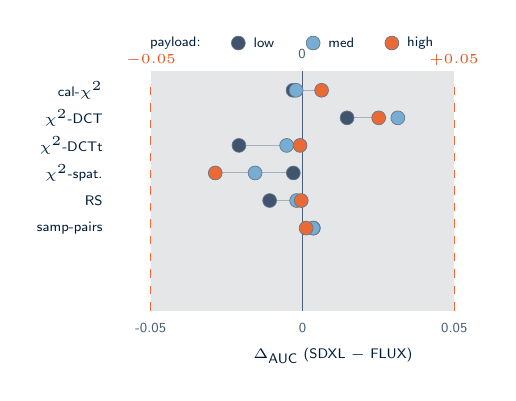
\begin{tikzpicture}[
  detrow/.style={font=\tiny\color{umdark}},
  dotlow/.style={circle, draw=umdark!60, fill=umdark!75,    inner sep=0pt, minimum size=5pt, line width=0.25pt},
  dotmed/.style={circle, draw=umdark!60, fill=umlight!75,   inner sep=0pt, minimum size=5pt, line width=0.25pt},
  dothigh/.style={circle, draw=umdark!60, fill=umorange!85, inner sep=0pt, minimum size=5pt, line width=0.25pt},
]
% RQ2 scale: Δ ∈ [-0.06, +0.08] → [0, 5.4] cm. Zero at x=2.31; ±0.05 at 0.39 / 4.24
\fill[umgray!18] (0.39,-2.85) rectangle (4.24,0.20);
\draw[umdark!70, line width=0.4pt] (2.31,-2.85) -- (2.31,0.20);
\node[font=\tiny\color{umdark!70}, above=1pt] at (2.31,0.20) {0};
\draw[umorange!85, line width=0.4pt, dashed] (0.39,-2.85) -- (0.39,0.10);
\draw[umorange!85, line width=0.4pt, dashed] (4.24,-2.85) -- (4.24,0.10);
\node[font=\tiny\color{umorange}, above=1pt] at (0.39,0.10) {$-0.05$};
\node[font=\tiny\color{umorange}, above=1pt] at (4.24,0.10) {$+0.05$};
\foreach \v in {-0.05,0,0.05} {
  \pgfmathsetmacro{\x}{(\v + 0.06) / 0.14 * 5.4}
  \node[font=\tiny\color{umdark!70}, below=1pt] at (\x,-2.85) {\v};
}
\node[font=\tiny\color{umdark}, below=10pt] at (2.7,-2.85) {$\Delta_\text{AUC}$ (SDXL $-$ FLUX)};

\foreach \i/\labl/\dl/\dm/\dh in {
  0/{cal-$\chi^2$}/-0.0031/-0.0021/0.0063,
  1/{$\chi^2$-DCT}/0.0147/0.0314/0.0251,
  2/{$\chi^2$-DCTt}/-0.0209/-0.0052/-0.0008,
  3/{$\chi^2$-spat.}/-0.0030/-0.0156/-0.0287,
  4/{RS}/-0.0108/-0.0019/-0.0004,
  5/{samp-pairs}/0.0036/0.0035/0.0012
} {
  \pgfmathsetmacro{\y}{-\i*0.35 - 0.05}
  \node[detrow, anchor=east] at (-0.10,\y) {\labl};
  \pgfmathsetmacro{\xa}{(\dl + 0.06) / 0.14 * 5.4}
  \pgfmathsetmacro{\xb}{(\dm + 0.06) / 0.14 * 5.4}
  \pgfmathsetmacro{\xcc}{(\dh + 0.06) / 0.14 * 5.4}
  \draw[umdark!35, line width=0.35pt] (\xa,\y) -- (\xcc,\y);
  \node[dotlow]  at (\xa,\y) {};
  \node[dotmed]  at (\xb,\y) {};
  \node[dothigh] at (\xcc,\y) {};
}
\node[font=\tiny\color{umdark}] at (0.7,0.55) {payload:};
\node[dotlow]  at (1.5,0.55) {};
\node[font=\tiny\color{umdark}, right=2pt] at (1.5,0.55) {low};
\node[dotmed]  at (2.45,0.55) {};
\node[font=\tiny\color{umdark}, right=2pt] at (2.45,0.55) {med};
\node[dothigh] at (3.45,0.55) {};
\node[font=\tiny\color{umdark}, right=2pt] at (3.45,0.55) {high};
\end{tikzpicture}
\end{center}
\vspace{-0.05cm}
{\scriptsize\color{umgray}Every dot sits inside the trivial band -- no SDXL\,$>$\,FLUX effect clears the $\delta_\text{min}\!=\!0.05$ threshold. The generators are interchangeable in their detector signature.}
\end{column}
\end{columns}
\end{frame}

% ============================================================
% 13b. Results: RQ2 -- per-stratum scatter
% ============================================================
\begin{frame}{RQ2 -- Per-Stratum AUC (SDXL vs.\ FLUX)}
\scriptsize
\begin{columns}[T]
\begin{column}{0.42\textwidth}
\begin{block}{Reading the plot}
\begin{itemize}\setlength{\itemsep}{1pt}
\item Each dot = one stratum (6 detectors $\times$ 3 payload levels = 18).
\item \textbf{Shape} = detector; \textbf{fill colour} = payload.
\item Dot on the diagonal $\Rightarrow$ generators equivalent for that stratum.
\item Orange band = $\pm 0.05$ practical margin.
\end{itemize}
\end{block}
\begin{exampleblock}{What to look for}
Every dot hugs the diagonal. \emph{Squares} ($\chi^2$-DCT) drift slightly toward SDXL-easier, \emph{stars} ($\chi^2$-DCT-tiled) and \emph{triangles} ($\chi^2$-spat.) the other way; max gap $\approx 0.03$, all inside the practical band.
\end{exampleblock}
\end{column}
\begin{column}{0.54\textwidth}
\begin{center}
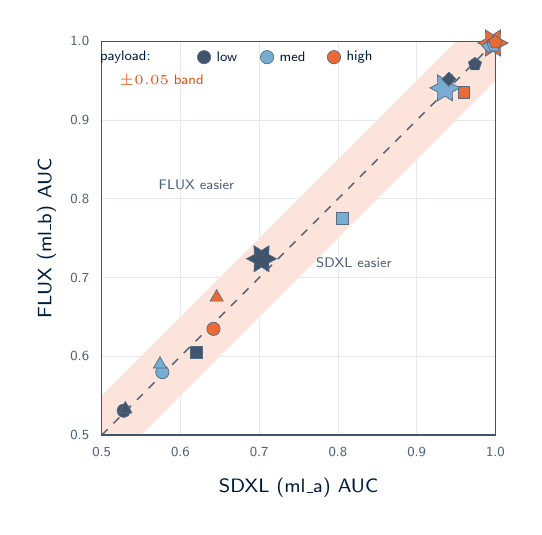
\begin{tikzpicture}[
  mCircle/.style ={circle, draw=umdark!65, inner sep=0pt, minimum size=4.8pt, line width=0.25pt},
  mSquare/.style ={rectangle, draw=umdark!65, inner sep=0pt, minimum size=4.2pt, line width=0.25pt},
  mDiamond/.style={diamond, draw=umdark!65, inner sep=0pt, minimum width=5.2pt, minimum height=5.2pt, line width=0.25pt},
  mTri/.style    ={regular polygon, regular polygon sides=3, draw=umdark!65, inner sep=0pt, minimum size=5.5pt, line width=0.25pt},
  mPenta/.style  ={regular polygon, regular polygon sides=5, draw=umdark!65, inner sep=0pt, minimum size=5pt, line width=0.25pt},
  mStar/.style   ={star, star points=6, star point ratio=0.55, draw=umdark!65, inner sep=0pt, minimum size=6.0pt, line width=0.25pt},
]
\def\sz{5}
\foreach \v in {0.5,0.6,0.7,0.8,0.9,1.0} {
  \pgfmathsetmacro{\xy}{(\v - 0.5) * 10}
  \draw[umdark!10, line width=0.3pt] (0,\xy) -- (\sz,\xy);
  \draw[umdark!10, line width=0.3pt] (\xy,0) -- (\xy,\sz);
  \node[font=\tiny\color{umdark!70}, left=1pt] at (0,\xy) {\v};
  \node[font=\tiny\color{umdark!70}, below=1pt] at (\xy,0) {\v};
}
\fill[umorange!15] (0,0.5) -- (4.5,5) -- (5,5) -- (5,4.5) -- (0.5,0) -- (0,0) -- cycle;
\draw[umdark!70, line width=0.5pt, dashed] (0,0) -- (\sz,\sz);
\draw[umdark!75, line width=0.5pt] (0,0) rectangle (\sz,\sz);
\node[font=\scriptsize\color{umdark}, below=12pt] at (\sz/2, 0) {SDXL (ml\_a) AUC};
\node[font=\scriptsize\color{umdark}, rotate=90] at (-0.7, \sz/2) {FLUX (ml\_b) AUC};

\node[font=\tiny\color{umorange}, anchor=south west] at (0.10,4.30) {$\pm 0.05$ band};
\node[font=\tiny\color{umdark!70}, anchor=south west] at (2.6,2.0) {SDXL easier};
\node[font=\tiny\color{umdark!70}, anchor=south west] at (0.6,3.0) {FLUX easier};

% 18 dots: shape encodes detector, fill encodes payload
% cal-χ² (circle)
\node[mCircle, fill=umdark!75]  at ({(0.528-0.5)*10},{(0.531-0.5)*10}) {};
\node[mCircle, fill=umlight!75] at ({(0.577-0.5)*10},{(0.580-0.5)*10}) {};
\node[mCircle, fill=umorange!85] at ({(0.642-0.5)*10},{(0.635-0.5)*10}) {};
% χ²-DCT (square)
\node[mSquare, fill=umdark!75]  at ({(0.620-0.5)*10},{(0.605-0.5)*10}) {};
\node[mSquare, fill=umlight!75] at ({(0.806-0.5)*10},{(0.775-0.5)*10}) {};
\node[mSquare, fill=umorange!85] at ({(0.960-0.5)*10},{(0.935-0.5)*10}) {};
% χ²-DCT-tiled (star)
\node[mStar, fill=umdark!75]   at ({(0.703-0.5)*10},{(0.724-0.5)*10}) {};
\node[mStar, fill=umlight!75]  at ({(0.936-0.5)*10},{(0.941-0.5)*10}) {};
\node[mStar, fill=umorange!85] at ({(0.997-0.5)*10},{(0.998-0.5)*10}) {};
% χ²-spatial (triangle)
\node[mTri, fill=umdark!75]   at ({(0.530-0.5)*10},{(0.533-0.5)*10}) {};
\node[mTri, fill=umlight!75]  at ({(0.574-0.5)*10},{(0.590-0.5)*10}) {};
\node[mTri, fill=umorange!85] at ({(0.646-0.5)*10},{(0.675-0.5)*10}) {};
% RS (diamond)
\node[mDiamond, fill=umdark!75]  at ({(0.941-0.5)*10},{(0.952-0.5)*10}) {};
\node[mDiamond, fill=umlight!75] at ({(0.992-0.5)*10},{(0.994-0.5)*10}) {};
\node[mDiamond, fill=umorange!85] at ({(0.998-0.5)*10},{(0.999-0.5)*10}) {};
% sample-pairs (pentagon)
\node[mPenta, fill=umdark!75]  at ({(0.974-0.5)*10},{(0.971-0.5)*10}) {};
\node[mPenta, fill=umlight!75] at ({(0.998-0.5)*10},{(0.995-0.5)*10}) {};
\node[mPenta, fill=umorange!85] at ({(1.000-0.5)*10},{(0.999-0.5)*10}) {};

% Payload legend
\node[font=\tiny\color{umdark}] at (0.30,4.80) {payload:};
\node[mCircle, fill=umdark!75]  at (1.30,4.80) {};
\node[font=\tiny\color{umdark}, right=1pt] at (1.30,4.80) {low};
\node[mCircle, fill=umlight!75] at (2.10,4.80) {};
\node[font=\tiny\color{umdark}, right=1pt] at (2.10,4.80) {med};
\node[mCircle, fill=umorange!85] at (2.95,4.80) {};
\node[font=\tiny\color{umdark}, right=1pt] at (2.95,4.80) {high};
\end{tikzpicture}

\vspace{0.05cm}
{\tiny\color{umdark}\textbf{detectors}\hspace{0.2em}
 \tikz[baseline=-2pt]\node[circle, draw=umdark!65, fill=umdark!30, inner sep=0pt, minimum size=4.5pt, line width=0.25pt]{};\,cal-$\chi^2$\hspace{0.5em}
 \tikz[baseline=-2pt]\node[rectangle, draw=umdark!65, fill=umdark!30, inner sep=0pt, minimum size=3.8pt, line width=0.25pt]{};\,$\chi^2$-DCT\hspace{0.5em}
 \tikz[baseline=-2pt]\node[star, star points=6, star point ratio=0.55, draw=umdark!65, fill=umdark!30, inner sep=0pt, minimum size=5pt, line width=0.25pt]{};\,$\chi^2$-DCTt\hspace{0.5em}
 \tikz[baseline=-2pt]\node[regular polygon, regular polygon sides=3, draw=umdark!65, fill=umdark!30, inner sep=0pt, minimum size=5pt, line width=0.25pt]{};\,$\chi^2$-spat.\hspace{0.5em}
 \tikz[baseline=-2pt]\node[diamond, draw=umdark!65, fill=umdark!30, inner sep=0pt, minimum width=4.8pt, minimum height=4.8pt, line width=0.25pt]{};\,RS\hspace{0.5em}
 \tikz[baseline=-2pt]\node[regular polygon, regular polygon sides=5, draw=umdark!65, fill=umdark!30, inner sep=0pt, minimum size=4.5pt, line width=0.25pt]{};\,samp-pairs}
\end{center}
\end{column}
\end{columns}
\end{frame}

% ============================================================
% 14. Results: RQ3 (payload interaction)
% ============================================================
\begin{frame}{RQ3 -- Payload Interaction with Source}
\scriptsize
\begin{columns}[T]
\begin{column}{0.46\textwidth}
\begin{block}{Real $-$ ML AUC gap, by payload ($N\!=\!3{,}000$)}
\begin{itemize}\setlength{\itemsep}{1pt}
\item Low (0.05 bpp):    $\boldsymbol{-0.0486}$
\item Medium (0.15 bpp): $\boldsymbol{-0.0281}$
\item High (0.30 bpp):   $\boldsymbol{-0.0157}$
\item Trend: \textbf{monotone, magnitude \emph{decreasing} with payload}
\item Verdict: \textbf{supported}
\end{itemize}
\end{block}
\begin{exampleblock}{Why the gap shrinks at high payload}
At higher embedding rates the per-pixel modification noise dominates the carrier-source statistical fingerprint. The carrier-origin signal is strongest where the embedding signal is weakest -- exactly the operationally relevant regime.
\end{exampleblock}
\end{column}
\begin{column}{0.50\textwidth}
\begin{center}
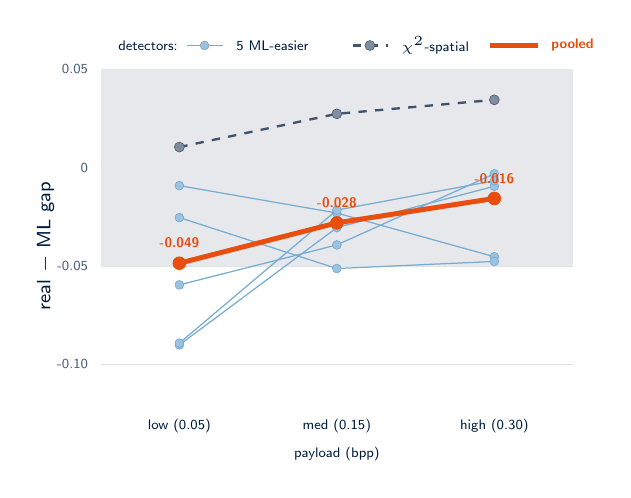
\begin{tikzpicture}[
  % All 4 ML-easier detectors share one muted shade so they read as the "cluster".
  detlineA/.style={line width=0.45pt, draw=umlight!75},
  detlineB/.style={line width=0.45pt, draw=umlight!75},
  % chi^2-spatial: visually distinct (dashed dark line) since it's the outlier.
  detlineC/.style={line width=0.85pt, draw=umdark!75, dashed},
  % Pooled: bold orange headline line.
  pooledline/.style={line width=1.8pt, draw=umorange},
  detmarkA/.style={circle, draw=umlight!80,  fill=umlight!55,  inner sep=0pt, minimum size=3.2pt, line width=0.2pt},
  detmarkB/.style={circle, draw=umlight!80,  fill=umlight!55,  inner sep=0pt, minimum size=3.2pt, line width=0.2pt},
  detmarkC/.style={circle, draw=umdark!75,   fill=umdark!50,   inner sep=0pt, minimum size=3.6pt, line width=0.2pt},
]
\def\xL{0}\def\xR{6}
\def\xlow{1}\def\xmed{3}\def\xhigh{5}
\foreach \v in {-0.10,-0.05,0,0.05} {
  \pgfmathsetmacro{\y}{(\v + 0.12) * 25}
  \draw[umdark!12, line width=0.3pt] (\xL,\y) -- (\xR,\y);
  \node[font=\tiny\color{umdark!70}, left=1pt] at (\xL,\y) {\v};
}
\pgfmathsetmacro{\yzero}{(0 + 0.12) * 25}
\draw[umdark!70, line width=0.4pt] (\xL,\yzero) -- (\xR,\yzero);
\pgfmathsetmacro{\ylo}{(-0.05 + 0.12) * 25}
\pgfmathsetmacro{\yhi}{(0.05 + 0.12) * 25}
\fill[umgray!16] (\xL,\ylo) rectangle (\xR,\yhi);

\node[font=\tiny\color{umdark}, below=2pt] at (\xlow,0)  {low (0.05)};
\node[font=\tiny\color{umdark}, below=2pt] at (\xmed,0)  {med (0.15)};
\node[font=\tiny\color{umdark}, below=2pt] at (\xhigh,0) {high (0.30)};
\node[font=\tiny\color{umdark}, below=12pt] at (\xmed,0) {payload (bpp)};
\node[font=\scriptsize\color{umdark}, rotate=90] at (-0.7,2.0) {real $-$ ML gap};

% Detector trends (unrolled to avoid foreach/style-key whitespace issues)
% Group A (umlight): cal-chi^2, chi^2-DCT, chi^2-DCT-tiled (all ML-easier)
\foreach \ll/\mm/\hh in {-0.0092/-0.0231/-0.0453, -0.0254/-0.0513/-0.0477, -0.0596/-0.0393/-0.0032} {
  \pgfmathsetmacro{\ya}{(\ll + 0.12) * 25}
  \pgfmathsetmacro{\yb}{(\mm + 0.12) * 25}
  \pgfmathsetmacro{\yc}{(\hh + 0.12) * 25}
  \draw[detlineA] (\xlow,\ya) -- (\xmed,\yb) -- (\xhigh,\yc);
  \node[detmarkA] at (\xlow,\ya)  {};
  \node[detmarkA] at (\xmed,\yb)  {};
  \node[detmarkA] at (\xhigh,\yc) {};
}
% Group B (umlight): rs, sample_pairs (also ML-easier)
\foreach \ll/\mm/\hh in {-0.0901/-0.0305/-0.0095, -0.0892/-0.0216/-0.0067} {
  \pgfmathsetmacro{\ya}{(\ll + 0.12) * 25}
  \pgfmathsetmacro{\yb}{(\mm + 0.12) * 25}
  \pgfmathsetmacro{\yc}{(\hh + 0.12) * 25}
  \draw[detlineB] (\xlow,\ya) -- (\xmed,\yb) -- (\xhigh,\yc);
  \node[detmarkB] at (\xlow,\ya)  {};
  \node[detmarkB] at (\xmed,\yb)  {};
  \node[detmarkB] at (\xhigh,\yc) {};
}
% Group C (umorange): chi^2-spatial (real-easier outlier)
{
  \pgfmathsetmacro{\ya}{(0.0104 + 0.12) * 25}
  \pgfmathsetmacro{\yb}{(0.0273 + 0.12) * 25}
  \pgfmathsetmacro{\yc}{(0.0344 + 0.12) * 25}
  \draw[detlineC] (\xlow,\ya) -- (\xmed,\yb) -- (\xhigh,\yc);
  \node[detmarkC] at (\xlow,\ya)  {};
  \node[detmarkC] at (\xmed,\yb)  {};
  \node[detmarkC] at (\xhigh,\yc) {};
}
\pgfmathsetmacro{\yp}{(-0.0486 + 0.12) * 25}
\pgfmathsetmacro{\yq}{(-0.0281 + 0.12) * 25}
\pgfmathsetmacro{\yr}{(-0.0157 + 0.12) * 25}
\draw[pooledline] (\xlow,\yp) -- (\xmed,\yq) -- (\xhigh,\yr);
\node[circle, draw=umorange, fill=umorange, inner sep=0pt, minimum size=4.5pt] at (\xlow,\yp)  {};
\node[circle, draw=umorange, fill=umorange, inner sep=0pt, minimum size=4.5pt] at (\xmed,\yq)  {};
\node[circle, draw=umorange, fill=umorange, inner sep=0pt, minimum size=4.5pt] at (\xhigh,\yr) {};
\node[font=\tiny\color{umorange}\bfseries, above=2pt] at (\xlow,\yp) {-0.049};
\node[font=\tiny\color{umorange}\bfseries, above=2pt] at (\xmed,\yq) {-0.028};
\node[font=\tiny\color{umorange}\bfseries, above=2pt] at (\xhigh,\yr) {-0.016};

\node[font=\tiny\color{umdark}, anchor=west] at (0.1, 4.55) {detectors:};
\draw[detlineA] (1.10,4.55) -- (1.55,4.55);
\node[detmarkA] at (1.32,4.55) {};
\node[font=\tiny\color{umdark}, anchor=west] at (1.60,4.55) {5 ML-easier};
\draw[detlineC] (3.20,4.55) -- (3.65,4.55);
\node[detmarkC] at (3.42,4.55) {};
\node[font=\tiny\color{umdark}, anchor=west] at (3.70,4.55) {$\chi^2$-spatial};
\draw[pooledline] (4.95,4.55) -- (5.55,4.55);
\node[font=\tiny\color{umorange}\bfseries, anchor=west] at (5.60,4.55) {pooled};
\end{tikzpicture}
\end{center}
\vspace{-0.05cm}
\end{column}
\end{columns}
\end{frame}

% ============================================================
% 15. Results: RQ4 (branch interaction)
% ============================================================
\begin{frame}{RQ4 -- Spatial vs.\ Frequency Branch}
\scriptsize
\begin{columns}[T]
\begin{column}{0.46\textwidth}
\begin{block}{(spatial gap $-$ frequency gap, $N\!=\!3{,}000$)}
\begin{itemize}\setlength{\itemsep}{1pt}
\item Pooled $\Delta\Delta_\text{AUC}$: $\boldsymbol{-0.0013}$ \\[1pt] (95\% CI $[-0.0031, +0.0005]$)
\item Strata with 95\% CI excluding 0: \textbf{2 / 3} (+1, $-$1)
\item Practically relevant ($|\Delta\Delta|\!\geq\!0.05$): 0 / 2
\item Verdict: \textbf{trivial} -- per-payload pattern persists (spatial wins at low, frequency at medium, tie at high) but pooled $\Delta\Delta$ is now indistinguishable from zero
\end{itemize}
\end{block}
\begin{exampleblock}{Per-payload pattern, pooled is trivial}
Spatial dominates at low ($-0.043$, practical), frequency at med ($+0.015$, trivial), tie at high ($-0.001$). The 3$\times$ sample tightens error bars; adding $\chi^2$-DCT-tiled to the frequency-branch average closes the pooled gap.
\end{exampleblock}
\end{column}
\begin{column}{0.50\textwidth}
\begin{center}
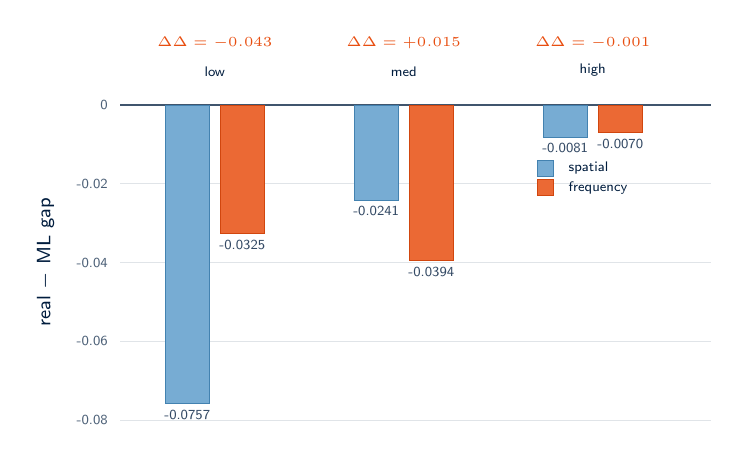
\begin{tikzpicture}[
  barlabel/.style={font=\tiny\color{umdark!80}},
  barspat/.style={draw=umlight!90!black, fill=umlight!75, line width=0.25pt},
  barfreq/.style={draw=umorange!90!black, fill=umorange!85, line width=0.25pt},
]
% y mapping: gap (negative) maps downward.  Range: -0.10 to +0.02 → -5..1 cm
% y_cm = val * 50  (so -0.10 → -5, 0 → 0, +0.02 → 1)
\def\xL{0}\def\xR{7.5}
% zero line + gridlines
\foreach \v in {-0.08,-0.06,-0.04,-0.02,0} {
  \pgfmathsetmacro{\y}{\v * 50}
  \draw[umdark!12, line width=0.3pt] (\xL,\y) -- (\xR,\y);
  \node[font=\tiny\color{umdark!70}, left=1pt] at (\xL,\y) {\v};
}
\draw[umdark!75, line width=0.5pt] (\xL,0) -- (\xR,0);
\node[font=\scriptsize\color{umdark}, rotate=90] at (-0.95,-2) {real $-$ ML gap};

% bar pairs per payload
\def\bw{0.55}
\def\bg{0.15}
\foreach \i/\pl/\spat/\freq/\dd in {
  0/{low}/-0.0757/-0.0325/{-0.043},
  1/{med}/-0.0241/-0.0394/{+0.015},
  2/{high}/-0.0081/-0.0070/{-0.001}
} {
  \pgfmathsetmacro{\xc}{1.2 + \i*2.4}
  \pgfmathsetmacro{\xa}{\xc - 0.5*\bw - \bg/2}
  \pgfmathsetmacro{\xb}{\xc + 0.5*\bw + \bg/2}
  \pgfmathsetmacro{\hspat}{\spat * 50}
  \pgfmathsetmacro{\hfreq}{\freq * 50}
  \draw[barspat] (\xa-\bw/2,0) rectangle (\xa+\bw/2,\hspat);
  \draw[barfreq] (\xb-\bw/2,0) rectangle (\xb+\bw/2,\hfreq);
  \node[barlabel, below=-1pt] at (\xa,\hspat) {\spat};
  \node[barlabel, below=-1pt] at (\xb,\hfreq) {\freq};
  \node[font=\tiny\color{umdark}, above=4pt] at (\xc,0.10) {\pl};
  \node[font=\tiny\color{umorange}\bfseries, above=14pt] at (\xc,0.10) {$\Delta\Delta=\dd$};
}

% Legend (top-right inside plot area, away from bars)
\begin{scope}[shift={(5.30, -1.20)}]
  \draw[barspat] (0,0.30) rectangle (0.20,0.50);
  \draw[barfreq] (0,0.05) rectangle (0.20,0.25);
  \node[font=\tiny\color{umdark}, right=2pt] at (0.20,0.40) {spatial};
  \node[font=\tiny\color{umdark}, right=2pt] at (0.20,0.15) {frequency};
\end{scope}
\end{tikzpicture}
\end{center}
\vspace{-0.05cm}
{\scriptsize\color{umgray}$\Delta\Delta$ = spatial gap $-$ frequency gap.}
\end{column}
\end{columns}
\end{frame}

% ============================================================
% 14. Results: RQ5
% ============================================================
\begin{frame}{RQ5 -- Encryption Invariance (verification)}
\scriptsize
\begin{columns}[T]
\begin{column}{0.46\textwidth}
\begin{block}{Test}
Paired DeLong between plain and AES-256-CBC stego on shared cover groups. Equivalence margin $\pm 0.025$ AUC per stratum.
\end{block}
\begin{block}{Headline finding ($N\!=\!3{,}000$)}
\begin{itemize}\setlength{\itemsep}{1pt}
\item Strata within $\pm 0.025$: \textbf{54 / 54}
\item Pooled $\Delta_\text{AUC}$: $\boldsymbol{-5.7\!\times\!10^{-7}}$ (95\% CI $\approx 0$)
\item Verdict: \textbf{supported -- encryption is invariant}
\end{itemize}
\end{block}
\begin{exampleblock}{Why the null matters}
A non-null result would indicate the detectors are reacting to payload structure rather than the embedding distortion itself. The clean null confirms the detectors respond to embedding artefacts, not plaintext patterns.
\end{exampleblock}
\end{column}
\begin{column}{0.50\textwidth}
\begin{center}
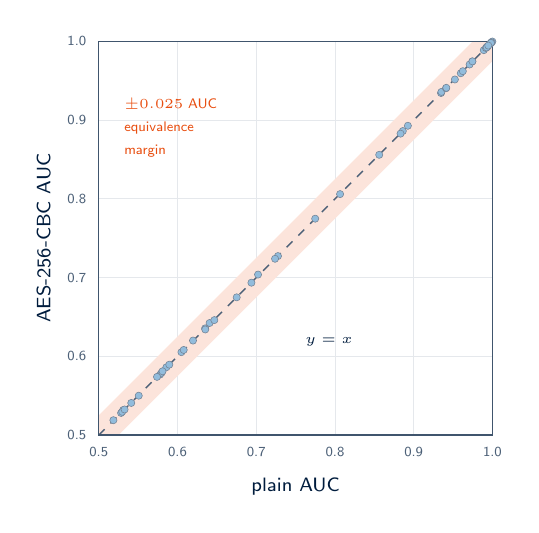
\begin{tikzpicture}[
  pt/.style={circle, draw=umdark!55, fill=umlight!60, inner sep=0pt, minimum size=2.6pt, line width=0.20pt},
]
% Plot area: AUC range [0.5, 1.0] mapped to [0, 5] cm for both axes.
\def\sz{5}
% Background grid
\foreach \v in {0.5,0.6,0.7,0.8,0.9,1.0} {
  \pgfmathsetmacro{\xy}{(\v - 0.5) * 10}
  \draw[umdark!10, line width=0.3pt] (0,\xy) -- (\sz,\xy);
  \draw[umdark!10, line width=0.3pt] (\xy,0) -- (\xy,\sz);
  \node[font=\tiny\color{umdark!70}, left=1pt] at (0,\xy) {\v};
  \node[font=\tiny\color{umdark!70}, below=1pt] at (\xy,0) {\v};
}
% ±0.025 equivalence band (parallel to identity)
\fill[umorange!15] (0,0.25) -- (4.75,5) -- (5,5) -- (5,4.75) -- (0.25,0) -- (0,0) -- cycle;
% Identity line
\draw[umdark!70, line width=0.5pt, dashed] (0,0) -- (\sz,\sz);
% Axes
\draw[umdark!75, line width=0.5pt] (0,0) rectangle (\sz,\sz);
\node[font=\scriptsize\color{umdark}, below=12pt] at (\sz/2, 0) {plain AUC};
\node[font=\scriptsize\color{umdark}, rotate=90] at (-0.7, \sz/2) {AES-256-CBC AUC};

% 54 points (6 detectors x 3 sources x 3 payloads = 54 strata)
\foreach \px/\py in {
  0.6408/0.6424, 0.6351/0.6356, 0.5859/0.5862, 0.5284/0.5282, 0.5310/0.5318, 0.5186/0.5190,
  0.5779/0.5769, 0.5798/0.5792, 0.5508/0.5501, 0.9598/0.9596, 0.9347/0.9345, 0.8926/0.8929,
  0.6197/0.6201, 0.6050/0.6054, 0.5810/0.5811, 0.8065/0.8061, 0.7749/0.7749, 0.7276/0.7274,
  0.9969/0.9970, 0.9979/0.9977, 0.9929/0.9932, 0.7023/0.7039, 0.7239/0.7240, 0.6353/0.6342,
  0.9352/0.9359, 0.9410/0.9405, 0.8862/0.8862, 0.6468/0.6461, 0.6752/0.6750, 0.6939/0.6936,
  0.5298/0.5296, 0.5328/0.5326, 0.5413/0.5409, 0.5740/0.5740, 0.5896/0.5895, 0.6079/0.6082,
  0.9983/0.9983, 0.9987/0.9987, 0.9890/0.9889, 0.9414/0.9411, 0.9523/0.9517, 0.8562/0.8560,
  0.9917/0.9917, 0.9938/0.9934, 0.9624/0.9622, 0.9999/0.9999, 0.9988/0.9988, 0.9927/0.9924,
  0.9744/0.9746, 0.9710/0.9707, 0.8833/0.8829, 0.9981/0.9981, 0.9947/0.9947, 0.9746/0.9747
} {
  \pgfmathsetmacro{\xx}{(\px - 0.5) * 10}
  \pgfmathsetmacro{\yy}{(\py - 0.5) * 10}
  \node[pt] at (\xx,\yy) {};
}
% Legend / annotation
\node[font=\tiny\color{umorange}, anchor=south west] at (0.2,4.0) {$\pm 0.025$ AUC};
\node[font=\tiny\color{umorange}, anchor=south west] at (0.2,3.7) {equivalence};
\node[font=\tiny\color{umorange}, anchor=south west] at (0.2,3.4) {margin};
\node[font=\tiny\color{umdark}, anchor=south west] at (2.5,1.0) {$y = x$};
\end{tikzpicture}
\end{center}
\vspace{-0.05cm}
\end{column}
\end{columns}
\end{frame}

% ============================================================
% 14b. Supplementary: pAUC analysis -- text + comparison
% ============================================================
\begin{frame}{Supplementary -- Partial AUC at FPR $\leq 0.10$}
\scriptsize
\begin{columns}[T]
\begin{column}{0.42\textwidth}
\begin{block}{Why pAUC, why FPR $\leq 0.10$?}
Full AUC integrates the entire ROC, including FPR regions a real steganalyst would never deploy. \textbf{pAUC} captures only the operationally relevant left tail. FPR $\leq 0.10$: standard since McClish (1989), matches the steganalysis screening regime, and fits the shape of our ROC curves.
\end{block}
\begin{exampleblock}{What changes under pAUC ($N\!=\!3{,}000$)}
\begin{itemize}\setlength{\itemsep}{1pt}
\item Effects \textbf{4--20$\times$ larger}: sample-pairs/low jumps from $-0.09$ (full) to $\boldsymbol{-0.30}$ (pAUC).
\item \textbf{RQ1: mixed $\to$ supported}; RQ2: trivial $\to$ mixed.
\item $\chi^2$-spatial flip \emph{dissolves} (all 3 strata $\leq|0.007|$, NS).
\end{itemize}
\end{exampleblock}
\end{column}
\begin{column}{0.54\textwidth}
\begin{block}{Verdict comparison (pre-reg.\ $\delta_\text{min}\!=\!0.05$)}
\centering\renewcommand{\arraystretch}{1.0}
\begin{tabular}{l@{\hskip 6pt}c@{\hskip 6pt}c}
& \textbf{full AUC} & \textbf{pAUC@FPR$\leq$0.10} \\
\midrule
\textbf{RQ1 (real vs ML)}   & mixed  & \textbf{supported} \\
\quad pooled $\Delta$    & $-0.0129$ & $-0.0174$ \\
\quad sig.~/~practical   & 16/18 ; 4/16 & 12/18 ; \textbf{6/12} \\
\midrule
\textbf{RQ2 (SDXL vs FLUX)} & trivial & \textbf{mixed} \\
\quad pooled $\Delta$    & $+0.0004$ & $+0.0008$ \\
\quad sig.~/~practical   & 7/18 ; 0/7 & 7/18 ; \textbf{1/7} \\
\end{tabular}
\end{block}
\begin{block}{Top RQ1 $|\Delta\text{-pAUC}|$ strata}
\scriptsize sample-pairs/lsb/low: $\boldsymbol{-0.30}$ \,$\cdot$\, rs/lsb/low: $-0.16$ \,$\cdot$\, sample-pairs/lsb/med: $-0.11$ \,$\cdot$\, rs/lsb/med: $-0.09$ \,$\cdot$\, $\chi^2$-DCT-tiled/dct/med: $-0.06$ \,$\cdot$\, $\chi^2$-DCT/dct/high: $-0.06$
\end{block}
\end{column}
\end{columns}
\end{frame}

% ============================================================
% 14c. Supplementary: pAUC scatter
% ============================================================
\begin{frame}{Supplementary -- RQ1 Per-Stratum pAUC@FPR$\leq$0.10}
\scriptsize
\begin{columns}[T]
\begin{column}{0.42\textwidth}
\begin{block}{Reading the plot}
\begin{itemize}\setlength{\itemsep}{1pt}
\item Each dot = one stratum (6 detectors $\times$ 3 payload levels = 18).
\item \textbf{Shape} = detector; \textbf{fill colour} = payload.
\item Above the diagonal $\Rightarrow$ ML easier at low FPR.
\item Orange band = $\pm 0.05$ practical margin.
\end{itemize}
\end{block}
\begin{exampleblock}{Same dots, sharper picture ($N\!=\!3{,}000$)}
The points spread \emph{much further} from the diagonal than under full AUC: sample-pairs/low and rs/low sit deep in the ML-easier zone (pAUC gap up to $0.30$). The 3 triangles ($\chi^2$-spat.) collapse back onto the diagonal -- the diffusion-flatness effect was a high-FPR artifact.
\end{exampleblock}
\end{column}
\begin{column}{0.54\textwidth}
\begin{center}
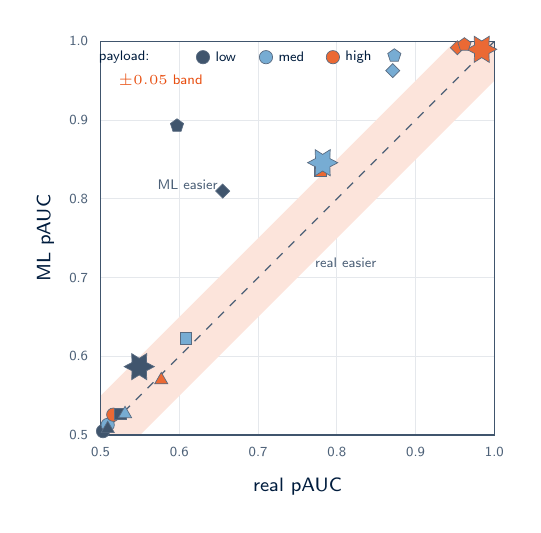
\begin{tikzpicture}[
  mCircle/.style ={circle, draw=umdark!65, inner sep=0pt, minimum size=4.8pt, line width=0.25pt},
  mSquare/.style ={rectangle, draw=umdark!65, inner sep=0pt, minimum size=4.2pt, line width=0.25pt},
  mDiamond/.style={diamond, draw=umdark!65, inner sep=0pt, minimum width=5.2pt, minimum height=5.2pt, line width=0.25pt},
  mTri/.style    ={regular polygon, regular polygon sides=3, draw=umdark!65, inner sep=0pt, minimum size=5.5pt, line width=0.25pt},
  mPenta/.style  ={regular polygon, regular polygon sides=5, draw=umdark!65, inner sep=0pt, minimum size=5pt, line width=0.25pt},
  mStar/.style   ={star, star points=6, star point ratio=0.55, draw=umdark!65, inner sep=0pt, minimum size=6.0pt, line width=0.25pt},
]
\def\sz{5}
\foreach \v in {0.5,0.6,0.7,0.8,0.9,1.0} {
  \pgfmathsetmacro{\xy}{(\v - 0.5) * 10}
  \draw[umdark!10, line width=0.3pt] (0,\xy) -- (\sz,\xy);
  \draw[umdark!10, line width=0.3pt] (\xy,0) -- (\xy,\sz);
  \node[font=\tiny\color{umdark!70}, left=1pt] at (0,\xy) {\v};
  \node[font=\tiny\color{umdark!70}, below=1pt] at (\xy,0) {\v};
}
\fill[umorange!15] (0,0.5) -- (4.5,5) -- (5,5) -- (5,4.5) -- (0.5,0) -- (0,0) -- cycle;
\draw[umdark!70, line width=0.5pt, dashed] (0,0) -- (\sz,\sz);
\draw[umdark!75, line width=0.5pt] (0,0) rectangle (\sz,\sz);
\node[font=\scriptsize\color{umdark}, below=12pt] at (\sz/2, 0) {real pAUC};
\node[font=\scriptsize\color{umdark}, rotate=90] at (-0.7, \sz/2) {ML pAUC};

\node[font=\tiny\color{umdark!70}, anchor=south west] at (2.6,2.0) {real easier};
\node[font=\tiny\color{umdark!70}, anchor=south west] at (0.6,3.0) {ML easier};
\node[font=\tiny\color{umorange}, anchor=south west] at (0.10,4.30) {$\pm 0.05$ band};

% 18 dots: shape encodes detector, fill encodes payload
% cal-χ² (circle)
\node[mCircle, fill=umdark!75]   at ({(0.503-0.5)*10},{(0.505-0.5)*10}) {};
\node[mCircle, fill=umlight!75]  at ({(0.509-0.5)*10},{(0.513-0.5)*10}) {};
\node[mCircle, fill=umorange!85] at ({(0.516-0.5)*10},{(0.526-0.5)*10}) {};
% χ²-DCT (square)
\node[mSquare, fill=umdark!75]   at ({(0.525-0.5)*10},{(0.527-0.5)*10}) {};
\node[mSquare, fill=umlight!75]  at ({(0.608-0.5)*10},{(0.623-0.5)*10}) {};
\node[mSquare, fill=umorange!85] at ({(0.779-0.5)*10},{(0.836-0.5)*10}) {};
% χ²-DCT-tiled (star)
\node[mStar, fill=umdark!75]    at ({(0.549-0.5)*10},{(0.587-0.5)*10}) {};
\node[mStar, fill=umlight!75]   at ({(0.782-0.5)*10},{(0.846-0.5)*10}) {};
\node[mStar, fill=umorange!85]  at ({(0.984-0.5)*10},{(0.990-0.5)*10}) {};
% χ²-spatial (triangle)
\node[mTri, fill=umdark!75]   at ({(0.509-0.5)*10},{(0.508-0.5)*10}) {};
\node[mTri, fill=umlight!75]  at ({(0.531-0.5)*10},{(0.527-0.5)*10}) {};
\node[mTri, fill=umorange!85] at ({(0.577-0.5)*10},{(0.570-0.5)*10}) {};
% RS (diamond)
\node[mDiamond, fill=umdark!75]   at ({(0.655-0.5)*10},{(0.810-0.5)*10}) {};
\node[mDiamond, fill=umlight!75]  at ({(0.871-0.5)*10},{(0.963-0.5)*10}) {};
\node[mDiamond, fill=umorange!85] at ({(0.953-0.5)*10},{(0.992-0.5)*10}) {};
% sample-pairs (pentagon)
\node[mPenta, fill=umdark!75]   at ({(0.597-0.5)*10},{(0.893-0.5)*10}) {};
\node[mPenta, fill=umlight!75]  at ({(0.873-0.5)*10},{(0.982-0.5)*10}) {};
\node[mPenta, fill=umorange!85] at ({(0.962-0.5)*10},{(0.996-0.5)*10}) {};

% Payload legend
\node[font=\tiny\color{umdark}] at (0.30,4.80) {payload:};
\node[mCircle, fill=umdark!75]   at (1.30,4.80) {};
\node[font=\tiny\color{umdark}, right=1pt] at (1.30,4.80) {low};
\node[mCircle, fill=umlight!75]  at (2.10,4.80) {};
\node[font=\tiny\color{umdark}, right=1pt] at (2.10,4.80) {med};
\node[mCircle, fill=umorange!85] at (2.95,4.80) {};
\node[font=\tiny\color{umdark}, right=1pt] at (2.95,4.80) {high};
\end{tikzpicture}

\vspace{0.05cm}
{\tiny\color{umdark}\textbf{detectors}\hspace{0.2em}
 \tikz[baseline=-2pt]\node[circle, draw=umdark!65, fill=umdark!30, inner sep=0pt, minimum size=4.5pt, line width=0.25pt]{};\,cal-$\chi^2$\hspace{0.5em}
 \tikz[baseline=-2pt]\node[rectangle, draw=umdark!65, fill=umdark!30, inner sep=0pt, minimum size=3.8pt, line width=0.25pt]{};\,$\chi^2$-DCT\hspace{0.5em}
 \tikz[baseline=-2pt]\node[star, star points=6, star point ratio=0.55, draw=umdark!65, fill=umdark!30, inner sep=0pt, minimum size=5pt, line width=0.25pt]{};\,$\chi^2$-DCTt\hspace{0.5em}
 \tikz[baseline=-2pt]\node[regular polygon, regular polygon sides=3, draw=umdark!65, fill=umdark!30, inner sep=0pt, minimum size=5pt, line width=0.25pt]{};\,$\chi^2$-spat.\hspace{0.5em}
 \tikz[baseline=-2pt]\node[diamond, draw=umdark!65, fill=umdark!30, inner sep=0pt, minimum width=4.8pt, minimum height=4.8pt, line width=0.25pt]{};\,RS\hspace{0.5em}
 \tikz[baseline=-2pt]\node[regular polygon, regular polygon sides=5, draw=umdark!65, fill=umdark!30, inner sep=0pt, minimum size=4.5pt, line width=0.25pt]{};\,samp-pairs}
\end{center}
\end{column}
\end{columns}
\end{frame}

% ============================================================
% 15. Limitations
% ============================================================
\section{Limitations}
\begin{frame}{Limitations}
\small
\begin{columns}[T]
\begin{column}{0.49\textwidth}
\begin{block}{Acknowledged deviations}
\begin{itemize}
\item ml\_b: PixArt-$\alpha$ replaced with FLUX.1-schnell (PixArt unavailable on HF Inference API).
\item Payload fill rates revised to $\{0.05, 0.15, 0.30\}$ to avoid detector saturation at the proposal's original $\{0.25, 0.50, 0.75\}$; the lower regime is operationally more realistic and lets the carrier-source signal emerge across the full detector family.
\item Verdicts shown are from the \textbf{$N\!=\!3{,}000$ confirmatory run}; the $N\!=\!1{,}000$ pre-registered run reproduces every direction with the single tightening of RQ4 from mixed to trivial (CI now spans zero).
\end{itemize}
\end{block}
\end{column}
\begin{column}{0.49\textwidth}
\begin{block}{Scope-bounded}
\begin{itemize}
\item Two generator families only -- cannot disentangle architecture from training data in RQ2.
\item Grayscale only; no colour information.
\item Classical detectors only; no learned baselines.
\item RQ4 pools over an asymmetric set (3 spatial vs 2 frequency detectors); the branch contrast accounts for this in its inverse-variance weighting.
\end{itemize}
\end{block}
\end{column}
\end{columns}
\end{frame}

% ============================================================
% 16. Contribution
% ============================================================
\section{Contribution}
\begin{frame}{Contribution and Minimum Deliverable}
\small
\begin{block}{What this study contributes}
\begin{itemize}
\item Caption-matched dataset across three carrier sources under identical embedding.
\item Training-free AUC-based comparison with DeLong and Holm correction.
\item Pre-computed RQ verdicts and power analysis as reproducible artefacts.
\end{itemize}
\end{block}
\begin{block}{Minimum deliverable met}
\begin{itemize}
\item One encryption scheme (AES-256-CBC). \checkmark
\item Two embedding approaches: spatial LSB and frequency DCT-LSB. \checkmark
\item Defensible answers to RQ1 and RQ2. \checkmark
\end{itemize}
\end{block}
\end{frame}

% ============================================================
% 16b. Phase 3 -- Extensions
% ============================================================
\begin{frame}{Phase 3 -- Extensions}
\scriptsize
\begin{columns}[T]
\begin{column}{0.49\textwidth}
\begin{block}{Completed since midway}
\begin{itemize}\setlength{\itemsep}{1pt}
\item \textbf{$N\!=\!3{,}000$ confirmatory run} -- 3$\times$ larger sample with 6 detectors and the same factorial; verdicts above reflect this run.
\end{itemize}
\end{block}
\begin{block}{Concrete next steps ($\sim$1 day each)}
\begin{itemize}\setlength{\itemsep}{1pt}
\item \textbf{Lower payload tier} (0.01 / 0.02 bpp) added to the factorial via \texttt{rerun\_with\_existing\_covers.py}; should widen the source gap on strong detectors.
\item \textbf{pAUC@FPR$\leq$0.10 as co-primary} -- promote the supplementary contrasts (slide 21) to a headline result.
\item \textbf{JPEG-quality sweep} (Q$\in\{75,85,95\}$): does the carrier-source effect survive lossy recompression?
\item \textbf{Vectorise the analysis pipeline} -- the $O(N^2)$ pure-Python ROC computation took $\sim$6\,h on the 648{,}000-row prediction set; \texttt{sklearn.metrics.roc\_curve} finishes the same work in seconds.
\end{itemize}
\end{block}
\end{column}
\begin{column}{0.49\textwidth}
\begin{block}{Mechanism investigations}
\begin{itemize}\setlength{\itemsep}{1pt}
\item \textbf{PoV-histogram skewness per source}: measure $\sum_k|n_{2k}-n_{2k+1}|$ on cover histograms of real vs.\ ML directly, with no embedding. Validates the diffusion-flatness explanation for the $\chi^2$-spatial flip.
\item \textbf{KL or MMD between source distributions vs.\ $\Delta_\text{AUC}$}: per detector, plot carrier-statistic distance against the observed effect size. Turns a per-detector heuristic story into a quantitative one.
\end{itemize}
\end{block}
\begin{block}{Smaller scope cleanups}
\begin{itemize}\setlength{\itemsep}{1pt}
\item Colour mode: store covers as YCbCr-Y instead of grayscale; detectors stay grayscale-equivalent but the carrier-statistic distance changes.
\item Promote the chi$^2$-spatial finding to a discussion paragraph in the report with the PoV-skewness evidence above.
\end{itemize}
\end{block}
\end{column}
\end{columns}
\end{frame}

% ============================================================
% 17. Closing
% ============================================================
\begin{frame}[plain]
\vfill
\begin{center}
{\color{umorange}\rule{0.32\textwidth}{2pt}}\\[14pt]
{\LARGE\bfseries\color{umdark}Thank you}\\[10pt]
{\large\color{umgray}Questions and Discussion}\\[16pt]
{\small\color{umgray}Code and run artefacts: \texttt{runs/<id>/}}\\[14pt]
{\color{umorange}\rule{0.32\textwidth}{2pt}}
\end{center}
\vfill
\end{frame}

\end{document}
